\documentclass{ieeeojies}
\usepackage{cite}
\usepackage{amsmath,amssymb,amsfonts}
\usepackage{algorithmic}
\usepackage{graphicx}
\usepackage{textcomp}
\usepackage{array}
\usepackage[table]{xcolor}
\definecolor{blue}{RGB}{47, 106, 255} % Define blue color
\usepackage{multirow}
\usepackage{multicol}
\usepackage{float}
\usepackage{indentfirst}
\usepackage{booktabs}
\usepackage{subcaption}
\usepackage[colorlinks=true, urlcolor=blue, linkcolor=red]{hyperref}
%\def\BibTeX{{\rm B\kern-.05em{\sc i\kern-.025em b}\kern-.08em
    %T\kern-.1667em\lower.7ex\hbox{E}\kern-.125emX}}

\begin{document}

\title{SOFWARE-INFRASTRUCTURE INDUSTRY STOCK PRICE PREDICTION USING STATISTICAL, MACHINE LEARNING AND DEEP LEARNING MODELS}

\author{
    \begin{tabular}{p{0.3\linewidth} p{0.3\linewidth} p{0.3\linewidth}}
        \centering\uppercase{Nguyen Thi Bich Dao}\authorrefmark{1} & \centering\uppercase{Le Nhat Binh}\authorrefmark{2} & \centering\uppercase{Le Tu}\authorrefmark{3}
    \end{tabular}
}

\address{
    \begin{tabular}{p{0.3\linewidth} p{0.3\linewidth} p{0.3\linewidth}}
        \centering Faculty of Information Systems, University of Information Technology, (e-mail: 21521925@gm.uit.edu.vn) & \centering Faculty of Information Systems, University of Information Technology, (e-mail: 21521875@gm.uit.edu.vn) & \centering Faculty of Information Systems, University of Information Technology, (e-mail: 21522738@gm.uit.edu.vn)
    \end{tabular}
}

\markboth
{Author \headeretal: Nguyen Thi Bich Dao, Le Nhat Binh, Le Tu}
{Author \headeretal: Nguyen Thi Bich Dao, Le Nhat Binh, Le Tu}

\begin{abstract}
The accurate prediction of stock price fluctuations holds significant importance for investors, publicly traded companies, and governmental bodies. The ongoing debate surrounding the feasibility of forecasting market trends has prompted this study to explore the efficacy of machine learning algorithms in predicting stock prices. Through the analysis of historical price data and pertinent features, various machine learning models including Linear Regression, ARIMA, RNN, GRU, LSTM, ETS, Meta-Learning, and AddRNN were trained and tested. The findings indicate that these algorithms can proficiently identify patterns and correlations within stock price data. As a result, the study concludes that machine learning algorithms hold significant promise as valuable tools for traders and investors navigating the dynamic and unpredictable nature of the stock market.
\end{abstract}

\begin{keywords}
Stock Price, Machine Learning, Time-Series, Forecasting.
\end{keywords}

\titlepgskip=-15pt

\maketitle

\section{Introduction}
\label{sec:introduction}
Predicting stock prices is always a significant challenge in the financial market. The accuracy of stock price forecasts plays a crucial role for investors in making investment decisions. In recent years, the use of algorithms for predicting stock prices has attracted considerable attention.

Algorithms have the ability to automatically learn from historical data and identify the best prediction models based on current and past data. This opens up opportunities to generate potential stock price forecasts. Based on this premise, the paper involves collecting stock data over 5 years from 2019 to 2024 from three companies in the software infrastructure sector: Adobe Inc, F5 Inc, and Akamai Technologies Inc. 

The data are used to forecast stock prices for the next 30, 60, and 90 days by using various algorithms including linear regression, ARIMA, RNN, GRU, LSTM, ETS, Meta-Learning, and AddRNN. From the forecasting results, we provide investors, traders and financial analysts with valuable insights and forecasts that can aid in making informed investment decisions. By accurately predicting future stock prices, investors can anticipate potential market movements and trends, thereby optimizing their investment strategies.


\section{Related Works}

% In recent years, there has been a substantial amount of research dedicated to predicting stock prices using various machine learning and statistical models.
% \\

% In a 2020 study, Zhanao, ZS, Sun \cite{b1} used exponential smoothing (ETS) and autoregressive integrated moving average (ARIMA) to forecast the trend of the S\&P 500 index close price data. The comparison of two models ARIMA and ETS have provided valuable insights into their respective strengths and weaknesses. By evaluating metrics such as mean error (ME), root mean squared error (RMSE), and mean absolute error (MAE), ARIMA models have smaller error values than those observed from ETS models, demonstrating a higher goodness of fit of ARIMA models. Forecasting result shows that the ARIMA model has a better performance with the data than the ETS models and can give a promising general trend prediction compared with existing methods.
% \\

% In the "Short-Term Stock Price-Trend Prediction Using Meta-Learning" \cite{b2} article, Shin-Hung Chang and his team used meta-learning framework with several convolutional neural networks, including the temporal convolution network, fully convolutional network, and residual neural network to predict the short-term stock price data. They use some label methods, Lunde and Pagan, are often used to identify market trends, which are not sensitive to high frequency short-term stock price trends and employed the proposed slope-detection method to define stock price trends, including “rise plus,” “rise,” “fall,” and “fall plus”. Authors approach meta-learning with two stage: meta-training and meta-testing. In addition, they use a long short-term memory (LSTM) neural network and the meta-learner is a model-agnostic meta-learning algorithm (MAML) as base learner. The authors also evaluated their approach on compared it with several baseline methods, including traditional machine learning models and deep learning models without meta-learning.
% \\

% % Yang Li and et al.\cite{b3} realized that there are factors influencing stock prices, including supply and demand dynamics, company news, economic factors, industry trends, market sentiment, and unexpected events. It emphasizes the importance of considering multiple factors for accurate stock price prediction. Previous approaches to stock price prediction often lacked comprehensive data and failed to account for factors like competitor information and time series analysis. They proposes a novel approach that integrates sentiment analysis with deep learning models, specifically LSTM and GRU networks, to improve prediction accuracy by considering both textual data and historical information. The result of the experiment show that the blending ensemble model attains 67\% accuracy in predicting stock movement directions, which is considered valuable for investment decision-making according to industry sources. 
% \\

% The paper "A recurrent neural network approach in predicting daily stock prices: An application to the Sri Lankan stock market" by A.J.P. Samarawickrama and T.G.I. Fernando discusses using recurrent neural networks (RNNs) to forecast daily stock prices. It compares feedforward networks, Simple RNN (SRNN), Gated Recurrent Unit (GRU), and Long Short-Term Memory (LSTM) networks, using past two days’ stock prices as inputs. Results show that while feedforward networks had high errors, they also achieved high accuracy in the best cases (99\%). SRNN and LSTM generally performed better than feedforward networks, while GRU had higher errors. The study concludes that RNN models might perform better with more input data.
% \\

% The paper "Predicting Prices of Stock Market using Gated Recurrent Units (GRUs) Neural Networks". The paper proposes a model to predict stock prices using Gated Recurrent Units (GRUs) neural networks, modified to avoid local minima, reduce time complexity, and enhance efficiency. By employing mini-batch gradient descent, the model balances the benefits of stochastic and batch gradient descents. The model's performance was evaluated using root mean square error (MSE) on various datasets, demonstrating successful and accurate stock price predictions. Future work aims to develop intelligent trading agents and automated trading bots for better decision-making and efficiency in trading.
% \\

% "Comparison of ARIMA, ANN and LSTM for Stock Price Prediction". The paper explores the prediction of stock prices using three different models: the autoregressive integrated moving average (ARIMA), artificial neural networks (ANN), and long short-term memory (LSTM) networks. It compares these models by analyzing their principles and prediction results. The study finds that while the LSTM model may have the best predictive capability, its performance is significantly influenced by data processing. The ANN model generally outperforms the ARIMA model, and integrating time series data with external factors could enhance predictions.
% \\

Recent years have seen increased research on stock price prediction using machine learning and statistical models.\\
A 2020 study by Zhanao, ZS, Sun\cite{b1} compared exponential smoothing (ETS) and autoregressive integrated moving average (ARIMA) models to forecast SP 500 index close prices. ARIMA models showed smaller error values and better performance in general trend prediction.\\
Shin-Hung Chang and colleagues used a meta-learning framework with convolutional neural networks (including temporal convolution network, fully convolutional network, and residual neural network) to predict short-term stock price trends\cite{b2}. They employed a slope-detection method to define trends and used long short-term memory (LSTM) neural networks with a model-agnostic meta-learning algorithm (MAML) as the base learner.\\
A study on the Sri Lankan stock market by Samarawickrama and Fernando \cite{b26} compared feedforward networks, Simple RNN (SRNN), Gated Recurrent Unit (GRU), and Long Short-Term Memory (LSTM) networks for daily stock price prediction. RNN models generally performed better, with SRNN and LSTM outperforming feedforward networks, while GRU had higher errors.\\
Another paper proposed using modified Gated Recurrent Units (GRU) neural networks for stock price prediction\cite{b5}. The model used mini-batch gradient descent to balance the benefits of stochastic and batch gradient descents. It showed successful and accurate predictions across various datasets.\\
A comparative study of ARIMA, Artificial Neural Networks (ANN), and LSTM models for stock price prediction found that while LSTM may have the best predictive capability, its performance is significantly influenced by data processing. ANN generally outperformed ARIMA, and the study suggested that integrating time series data with external factors could enhance predictions.\\
\section{Materials}
\subsection{Datasets}
The data used in the research project is historical stock price data of Adobe Inc, AKAM Inc, FFIV Inc provided on the website Finance.yahoo.com. Coverage period is from February 1, 2019 to March 25, 2019.
\begin{itemize}
  \item \textbf{Date} – Date
  \item \textbf{Open} – Opening price
  \item \textbf{High} – Highest price of the day
  \item \textbf{Low} – Lowest price of the day
  \item \textbf{Close} – Closing price
  \item \textbf{Adj Close} – The closing price adjusts for company actions however the virtual currency has no holding company so the adjusted closing price is equal to the closing price.
  \item \textbf{Volume} – Total trading volume for the day.
\end{itemize}
\subsubsection{Detail statistical}
\begin{table}[H]
    \centering
    \begin{tabular}{lccc}
        \toprule
        & \textbf{ADBE} & \textbf{AKAM} & \textbf{FFIV} \\
        \midrule
        Count & 1324000000 & 1324000000 & 1324000000 \\
        Mean & 437561171 & 98894456 & 163434992 \\
        Std & 112802864 & 13155544 & 29329932 \\
        Min & 254740005 & 69120003 & 90550003 \\
        25\% & 339532501 & 88715000 & 141537506 \\
        50\% & 443785004 & 100404999 & 155590004 \\
        75\% & 514142502 & 110002501 & 186022503 \\
        Max & 688369995 & 128320007 & 24779999 \\
        \bottomrule
    \end{tabular}
     \caption{Summary statistics for ADBE, AKAM, and FFIV}
    \label{tab:summary-stats}
\end{table}
\subsubsection{Visualize}
\paragraph{ADBE}
\begin{figure}[H]
    \begin{subfigure}{0.4\linewidth}
        \centering
        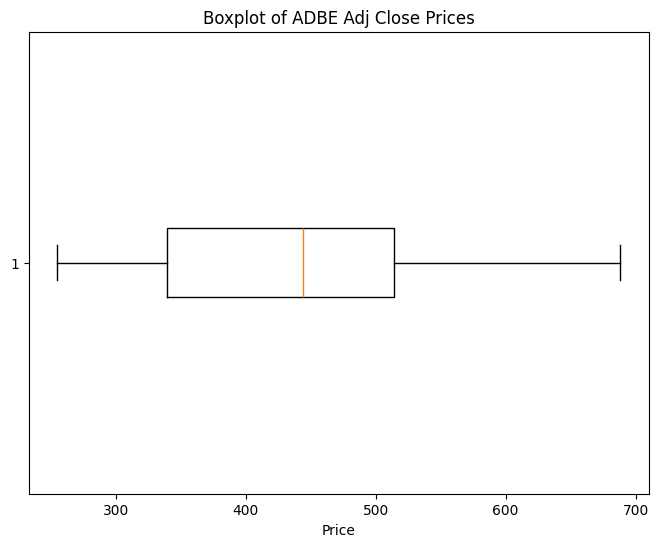
\includegraphics[width=\linewidth]{ADBE1.png}
        \caption{ADBE Boxplot}
        \label{fig:adbe-7-3}
    \end{subfigure}%
    \hfill
    \begin{subfigure}{0.4\linewidth}
        \centering
        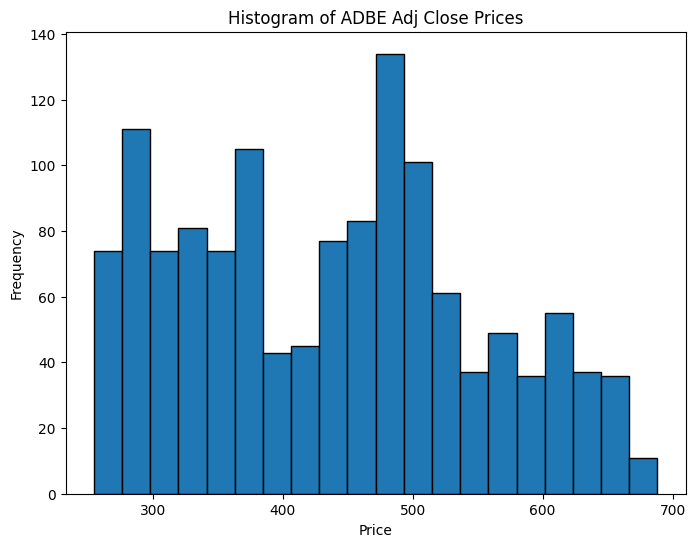
\includegraphics[width=\linewidth]{ADBE2.png}
        \caption{ADBE Histogram}
        \label{fig:adbe-8-2}
    \end{subfigure}%
\end{figure}
\paragraph{AKAM}
\begin{figure}[H]
    \begin{subfigure}{0.4\linewidth}
        \centering
        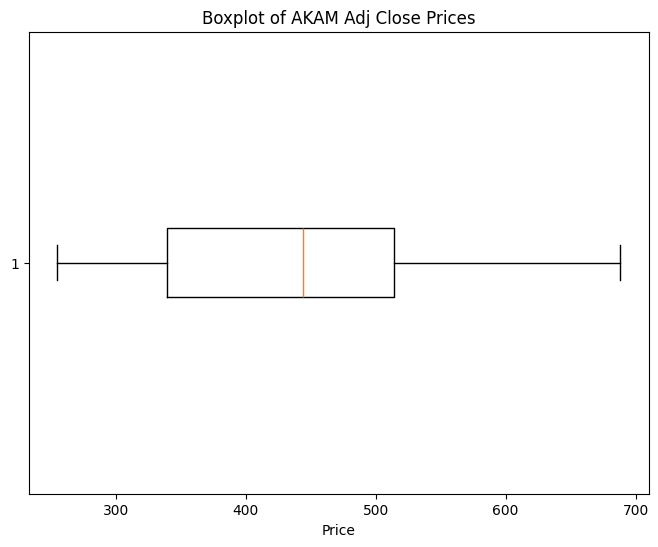
\includegraphics[width=\linewidth]{AKAM1.png}
        \caption{AKAM Boxplot}
        \label{fig:adbe-7-3}
    \end{subfigure}%
    \hfill
    \begin{subfigure}{0.4\linewidth}
        \centering
        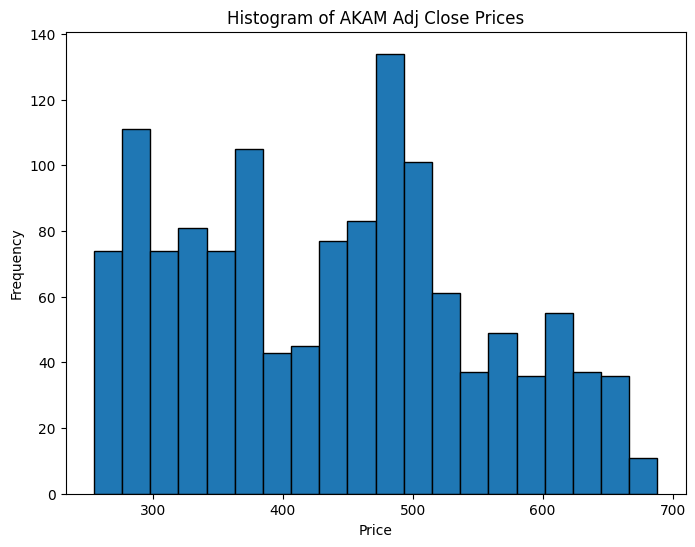
\includegraphics[width=\linewidth]{AKAM2.png}
        \caption{AKAM Histogram}
        \label{fig:adbe-8-2}
    \end{subfigure}%
\end{figure}
\paragraph{FFIV}
\begin{figure}[H]
    \begin{subfigure}{0.4\linewidth}
        \centering
        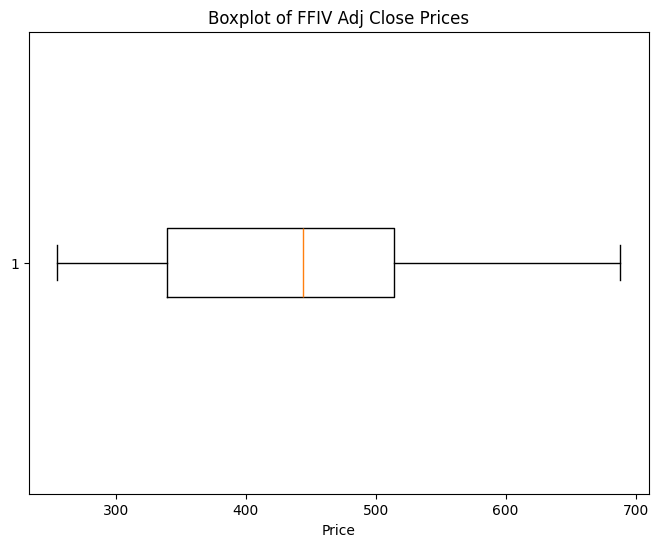
\includegraphics[width=\linewidth]{FFIV1.png}
        \caption{FFIV Boxplot}
        \label{fig:adbe-7-3}
    \end{subfigure}%
    \hfill
    \begin{subfigure}{0.4\linewidth}
        \centering
        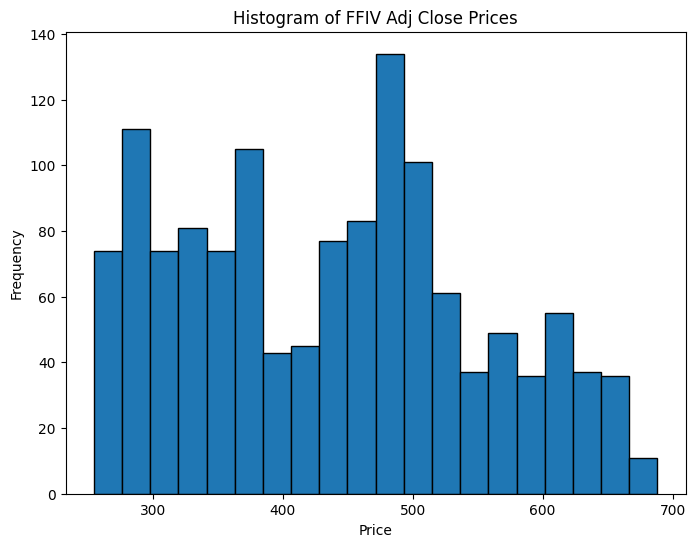
\includegraphics[width=\linewidth]{FFIV2.png}
        \caption{FFIV Histogram}
        \label{fig:adbe-8-2}
    \end{subfigure}%
\end{figure}
\subsection{Datasets Split Ratio}
In our research, we split data into train and test with ratios 8:2, 7:3 and 75:25 relatively. Both 7:3 and 8:2 are common ratios in machine learning. The 7:3 ratio offers a slightly larger test set, which can be advantageous for robust model evaluation and validation. This allocation ensures that the model's performance metrics are based on a substantial amount of unseen data, promoting confidence in its ability to generalize beyond the training set. On the other hand, the 8:2 ratio provides a more pronounced emphasis on training data, beneficial when aiming to maximize the model's learning potential with ample examples. This setup is particularly useful for complex models that require extensive data to capture intricate patterns and nuances effectively. Moreover, we also use 75:25 ratio to optimize both the training and evaluation processes, ensuring stability and effectiveness across various real-world applications.
\subsection{Model Evaluation Metrics}
Mean Absolute Percentage Error (MAPE) is a metric used to quantify the accuracy of a forecasting or prediction model. It measures the average absolute percentage difference between the forecasted values and the actual values. MAPE is expressed as a percentage, where lower values indicate better accuracy. 

\begin{equation}
\text{MAPE} = \frac{1}{N} \frac{1}{H} \sum_{i=1}^{N} \sum_{t=T+1}^{T+H} \frac{| y_{i,t} - f_{i,t} |}{| y_{i,t} |}
\end{equation}

Where:
\begin{itemize}
    \item \( N \) is the total number of observations,
    \item \( H \) is the forecast horizon,
    \item \( T \) is the total number of historical periods,
    \item \( y_{i,t} \) is the actual value at observation \( i \) and time \( t \),
    \item \( f_{i,t} \) is the forecasted value at observation \( i \) and time \( t \).
\end{itemize}


Root Mean Square Error (RMSE) is a measure of the differences between predicted values by a model or estimator and the actual values observed.  RMSE provides a single number to summarize the magnitude of errors in predictions, with lower values indicating better agreement between predicted and observed values.

\begin{equation}
\text{RMSE} = \sqrt{\frac{1}{N} \frac{1}{H} \sum_{i=1}^{N} \sum_{t=T+1}^{T+H} (y_{i,t} - f_{i,t})^2}
\end{equation}

Where:
\begin{itemize}
    \item \( N \) is the total number of observations,
    \item \( H \) is the forecast horizon,
    \item \( T \) is the total number of historical periods,
    \item \( y_{i,t} \) is the actual value at observation \( i \) and time \( t \),
    \item \( f_{i,t} \) is the forecasted value at observation \( i \) and time \( t \).
\end{itemize}

Mean Absolute Error (MAE) is a metric used to evaluate the accuracy of a predictive model by measuring the average absolute difference between predicted values and actual values. It provides a straightforward measure of prediction error that is easy to interpret and compare across different models or datasets.

\begin{equation}
\text{MAE} = \frac{1}{N} \frac{1}{H} \sum_{i=1}^{N} \sum_{t=T+1}^{T+H} \left| y_{i,t} - f_{i,t} \right|
\end{equation}

Where:
\begin{itemize}
    \item \( N \) is the total number of observations,
    \item \( H \) is the forecast horizon,
    \item \( T \) is the total number of historical periods,
    \item \( y_{i,t} \) is the actual value at observation \( i \) and time \( t \),
    \item \( f_{i,t} \) is the forecasted value at observation \( i \) and time \( t \).
\end{itemize}

\section{Methods}
\subsection{Linear Regression}
Linear regression is a statistical modeling technique used to determine the relationship between a dependent variable and one or more independent variables. The goal of linear regression is to find the best-fitting straight line that models the relationship between these variables.
\begin{equation}
y_t = \beta_0 + \beta_1 x_t + \epsilon_t
\end{equation}

Where:
\begin{itemize}
    \item \( y_t \) is the dependent variable at time \( t \),
    \item \( \beta_0 \) and \( \beta_1 \) are the intercept and slope coefficients,
    \item \( x_t \) is the independent variable at time \( t \),
    \item \( \epsilon_t \) is the error term at time \( t \).
\end{itemize}

\subsection{ARIMA}
An autoregressive integrated moving average (ARIMA) model is a statistical tool utilized for analyzing time series data, aimed at gaining deeper insights into the dataset or forecasting forthcoming trends.
ARIMA stands for autoregressive integrated moving average model and is specified by three order parameters: (p, d, q)
\begin{itemize}
    \item \textbf{AR(p) Autoregression}: A regression model that utilizes the dependent relationship between a current observation and observations over a previous period. An autoregressive (AR(p)) component refers to the use of past values in the regression equation for the time series:
    \begin{equation}
y_t = c + \phi_1 y_{t-1} + \phi_2 y_{t-2} + \ldots + \phi_p y_{t-p} + \epsilon_t,
\end{equation}

where:
\begin{itemize}
    \item \( y_t \) is the value of the time series at time \( t \),
    \item \( c \) is the constant term (intercept),
    \item \( \phi_1, \phi_2, \ldots, \phi_p \) are the autoregressive coefficients for lags 1 to \( p \),
    \item \( y_{t-1}, y_{t-2}, \ldots, y_{t-p} \) are the lagged values of the time series,
    \item \( \epsilon_t \) is the error term at time \( t \).
\end{itemize}
    
    \item \textbf{I(d) Integration}: Uses differencing of observations (subtracting an observation from observation at the previous time step) in order to make the time series stationary. Differencing involves the subtraction of the current values of a series with its previous values \( d \) number of times.
    
    \item \textbf{MA(q) Moving Average}: A model that uses the dependency between an observation and a residual error from a moving average model applied to lagged observations. A moving average component depicts the error of the model as a combination of previous error terms. The order \( q \) represents the number of terms to be included in the model.
    \begin{equation}
y_t = c + \epsilon_t + \theta_1 \epsilon_{t-1} + \theta_2 \epsilon_{t-2} + \ldots + \theta_q \epsilon_{t-q},
\end{equation}

where:
\begin{itemize}
    \item \( y_t \) is the value of the time series at time \( t \),
    \item \( c \) is the constant term (intercept),
    \item \( \epsilon_t \) is the error term at time \( t \),
    \item \( \theta_1, \theta_2, \ldots, \theta_q \) are the coefficients of the lagged error terms (\( \epsilon_{t-1}, \epsilon_{t-2}, \ldots, \epsilon_{t-q} \)).
\end{itemize}
\end{itemize}
So the equation of an ARIMA model becomes:
\begin{equation}
y_t = c + \epsilon_t + \phi_1 y_{t-1} + \phi_2 y_{t-2} + \ldots + \phi_p y_{t-p} + \theta_1 \epsilon_{t-1} + \theta_2 \epsilon_{t-2} + \ldots + \theta_q \epsilon_{t-q},
\end{equation}

\subsection{RNN}
A Recurrent Neural Network (RNN) is a type of artificial neural network designed to process sequential data by maintaining a form of internal state or memory. RNN is well-suited for tasks where the input's temporal order is important, such as time series prediction, natural language processing (NLP), and speech recognition.\\
Because unlike traditional feedforward neural networks, RNNs have connections that loop back on themselves, allowing information to persist across time steps. 
\begin{figure}
    \centering
    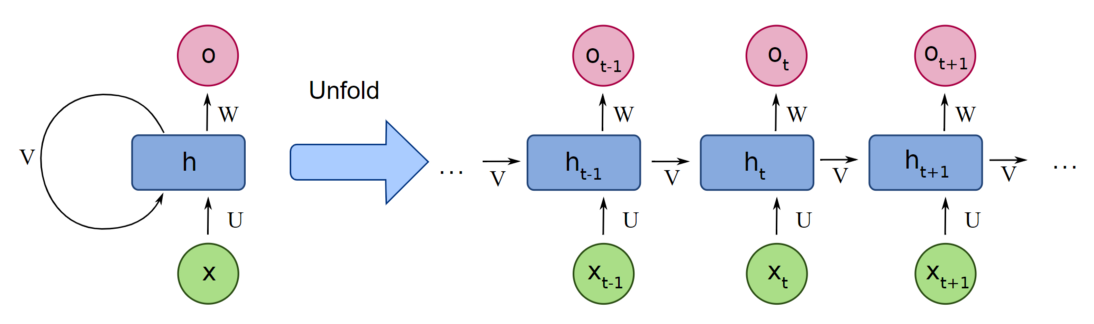
\includegraphics[width=0.5\linewidth]{image-80.png}
    \caption{How RNN works}
    \label{fig:enter-label}
\end{figure}
At each time step, the hidden state of the RNN is updated based on the current input and the previous hidden state, enabling the network to capture temporal dependencies in the data. The hidden state is computed using a weighted sum of the current input and the previous hidden state, passed through an activation function.
The hidden state \( h(t) \) is computed using the following formula:
\begin{equation}
h(t) = \sigma \left( W_{ih} x(t) + W_{hh} h(t-1) + b_h \right)
\end{equation}

where:
\begin{itemize}
    \item \( \sigma \) is an activation function (often \(\tanh\) or \(\mathrm{ReLU}\)).
    \item \( W_{ih} \) is the weight matrix for the input to hidden state.
    \item \( W_{hh} \) is the weight matrix for the hidden state to hidden state (recurrent weights).
    \item \( b_h \) is the bias term.
\end{itemize}

The output \( y(t) \) at each time step can be computed as:
\begin{equation}
y(t) = \phi \left( W_{ho} h(t) + b_o \right)
\end{equation}

where:
\begin{itemize}
    \item \( \phi \) is an activation function (often softmax for classification tasks).
    \item \( W_{ho} \) is the weight matrix from hidden state to output.
    \item \( b_o \) is the bias term for the output.
\end{itemize}

\subsection{LSTM}
LSTM, a type of recurrent neural network, overcomes the vanishing gradient problem found in traditional RNNs by incorporating additional cells, as well as input and output gates. Essentially, it addresses vanishing gradients by using additive components and forget gate activations, which enable gradients to propagate through the network more effectively without diminishing rapidly.
\begin{figure}[H]
  \centering
  \begin{minipage}{0.8\linewidth}
    \centering
    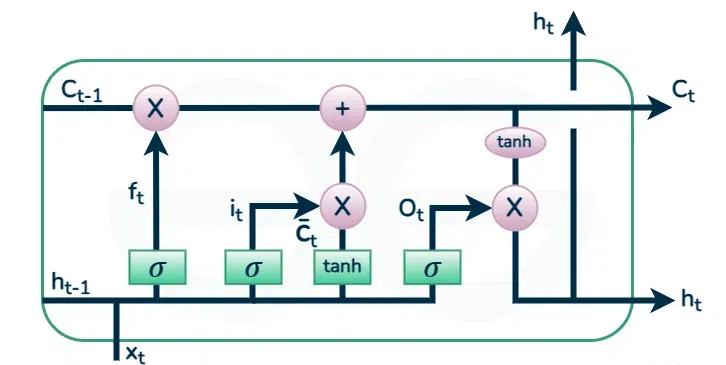
\includegraphics[width=\linewidth]{LSTM Plot/lstm.png}
    \caption{LSTM cell \cite{b12}}
    \label{fig2}
  \end{minipage}
\end{figure}
The LSTM structure includes a memory cell regulated by three gates: the input gate, the forget gate, and the output gate. These gates dictate which information is incorporated into the cell, erased from it, and transmitted as output from the memory cell.\cite{b12}

\begin{itemize}
    \item \textbf{Forget Gate:} Controls the removal of information from the cell state.
    \[
    f_t = \sigma(W_f \cdot [h_{t-1}, x_t] + b_f)
    \]
    where \( \sigma \) is the sigmoid activation function, \( W_f \) is the weight matrix associated with the forget gate, \( h_{t-1} \) is the previous hidden state, \( x_t \) is the current input, and \( b_f \) is the bias.
    
    \item \textbf{Input Gate:} Controls the addition of new information to the cell state.
    \[
    i_t = \sigma(W_i \cdot [h_{t-1}, x_t] + b_i)
    \]
    \[
    \widetilde{C}_t = \tanh(W_c \cdot [h_{t-1}, x_t] + b_c)
    \]
    where \( \widetilde{C}_t \) is the candidate cell state, \( \tanh \) is the hyperbolic tangent activation function, \( W_i \) and \( W_c \) are the weight matrices associated with the input gate and candidate cell state, and \( b_i \), \( b_c \) are biases.
    
    \item \textbf{Cell State Update:}
    \[
    C_t = f_t \odot C_{t-1} + i_t \odot \widetilde{C}_t
    \]
    where \( \odot \) denotes element-wise multiplication.
    
    \item \textbf{Output Gate:} Controls the extraction of useful information from the cell state to produce the output.
    \[
    o_t = \sigma(W_o \cdot [h_{t-1}, x_t] + b_o)
    \]
    \[
    h_t = o_t \odot \tanh(C_t)
    \]
    where \( h_t \) is the output of the LSTM cell, \( W_o \) are the weight matrix and \( b_o \) is the bias.
\end{itemize}
\subsection{GRU}
Gated Recurrent Units (GRU) are a specialized type of recurrent neural network (RNN) designed to efficiently capture relationships in sequential data. GRU simplify the complexity of traditional RNN by using gating mechanisms to regulate the flow of information.explores the application of GRU in predicting stock market prices, demonstrating their capability to model time-series data with high accuracy.The study highlights the GRU's advantages over other models, such as reduced computational cost and improved performance in capturing long-term dependencies in stock market trends.

Gated Recurrent Units (GRU) employ two crucial gates to manage the flow of information: the update gate and the reset gate.

\textbf{Update Gate}: Manages the extent to which the unit updates its content. It balances the retention of past information and the incorporation of new data, maintaining essential long-term information.

\textbf{Reset Gate}: Determines which information should be forgotten. This allows the model to reset its memory, focusing on relevant new inputs.

These mechanisms enable GRU to handle sequential data effectively, mitigating the vanishing gradient problem common in traditional recurrent neural networks (RNN).


\textbf{Hidden State and Formulas}\cite{b18}

The hidden state \( h_t \) in a GRU at time step \( t \) is a combination of the previous hidden state \( h_{t-1} \) and the current candidate hidden state \( \tilde{h}_t \), modulated by the update gate \( z_t \). The formulas for the update gate \( z_t \), the reset gate \( r_t \), and the candidate hidden state \( \tilde{h}_t \) are as follows\cite{}:

\begin{align}
z_t &= \sigma(W_z x_t + U_z h_{t-1} + b_z) \\
r_t &= \sigma(W_r x_t + U_r h_{t-1} + b_r) \\
\tilde{h}_t &= \tanh(W_h x_t + U_h (r_t \odot h_{t-1}) + b_h) \\
h_t &= (1 - z_t) \odot h_{t-1} + z_t \odot \tilde{h}_t
\end{align}

Where:

- \( z_t \) is the update gate vector.

- \( r_t \) is the reset gate vector.

- \( \tilde{h}_t \) is the candidate activation vector.

- \( \sigma \) is the sigmoid activation function.

- \( \tanh \) is the hyperbolic tangent activation function.

- \( W_z, W_r, W_h \) are the weight matrices for the input \( x_t \).

- \( U_z, U_r, U_h \) are the weight matrices for the hidden state \( h_{t-1} \).

- \( b_z, b_r, b_h \) are the bias vectors.

- \( \odot \) denotes element-wise multiplication.

- \( x_t \) is the input vector at time step \( t \).

- \( h_{t-1} \) is the hidden state vector from the previous time step.

These gates and the hidden state update mechanism allow GRU to adaptively capture and utilize relevant information from the sequence data.
\subsection{ETS}
ETS, also known as Error, Trend, and Seasonality models, are a class of exponential smoothing methods used for forecasting time series data. The ETS encompasses a variety of models that account for error, trend, and seasonal components in different ways. The ETS approach is distinct because it integrates these components within a State Space statistical framework, allowing for a more comprehensive understanding and modeling of the time series data. 
\textbf{Key Components of ETS Models}
\begin{itemize}
    \item \textbf{Error ($E$)}:  The error component can be additive (A) or multiplicative (M). It captures the unpredictable component of the data.
    \item \textbf{Trend ($T$)}: The trend component can be none (N), additive (A), additive damped (Ad), multiplicative (M), or multiplicative damped (Md). It represents the long-term direction in the data.
    \item \textbf{Seasonality ($L$)}: The seasonality component can be none (N), additive (A), or multiplicative (M). It captures periodic fluctuations. \cite{b8, b9}
\end{itemize}
The combination of ETS can be up to 30 models.


\begin{tabular}{@{}lll@{}}
\toprule
\textbf{Model} & \textbf{Model} & \textbf{Model} \\
\midrule
ETS (M, M, N) & ETS (A, M, A) & ETS (M, N, M) \\
ETS (M, A, N) & ETS (A, Md, N) & ETS (M, N, A) \\
ETS (A, M, N) & ETS (A, N, A) & ETS (M, N, N) \\
ETS (M, A, M) & ETS (A, Md, M) & ETS (M, A, A) \\
ETS (A, A, M) & ETS (M, Ad, M) & ETS (A, Ad, M) \\
ETS (A, N, N) & ETS (M, Ad, N) & ETS (M, M, A) \\
ETS (M, M, M) & ETS (M, Md, M) & ETS (A, A, A) \\
ETS (A, N, M) & ETS (A, Ad, N) & ETS (A, Ad, A) \\
ETS (A, A, N) & ETS (M, Md, A) & ETS (M, Ad, A) \\
ETS (A, M, M) & ETS (M, Md, N) & ETS (A, Md, A) \\
\bottomrule
\end{tabular}
\caption{ETS Models}

\noindent The state space models for all 30 Exponential Smoothing variations involves a state vector \cite{b9}:
\begin{align}
    \mathbf{x}_t &= (\ell_t, b_t, s_t, s_{t-1}, \ldots, s_{t-m+1})'
\end{align}
And state space equations of the form are as follow:
\begin{align}
    y_t &= w(\mathbf{x}_{t-1}) + r(\mathbf{x}_{t-1})\epsilon_t,  \\
    \mathbf{x}_t &= f(\mathbf{x}_{t-1}) + g(\mathbf{x}_{t-1})\epsilon_t, 
\end{align}

Where:
\begin{itemize}
    \item \( y_t \): observed value at time \( t \)
    \item \( \mathbf{x}_t \): state vector at time \( t \)
    \item \( \ell_t \): level component at time \( t \)
    \item \( b_t \): trend component at time \( t \)
    \item \( s_t \): seasonal component at time \( t \)
    \item \( s_{t-1}, \ldots, s_{t-m+1} \): previous seasonal components
    \item \( \epsilon_t \): Gaussian white noise process with variance \( \sigma^2 \)
    \item \( \mu_t \): mean level at time \( t \), defined as \( \mu_t = w(\mathbf{x}_{t-1}) \)
    \item \( r(\mathbf{x}_{t-1}) \): function defining the error structure
    \item \(f\): the transition
    \item \(g\): the persistence functions
\end{itemize}

From the ETS model combinations above, there are 15 models with additive errors and 15 models with multiplicative errors. In time series analysis, some models may satisfy the necessary assumptions. To determine the best model among the 30 ETS models, several criteria can be used, including Akaike's Information Criterion (AIC), Akaike's Information Criterion correction (AICc), and Bayesian Information Criterion (BIC)\cite{b9}.

Akaike's Information Criterion(AIC) can be calculated base on this formula:
\[
\text{AIC} = -2 \log(L) + 2k,
\]

The Akaike's Information Criterion correction (AICc) can be calculated by this formula:
\[
\text{AIC}_c = \text{AIC} + \frac{2k(k+1)}{T-k-1},
\]
and the Bayesian Information Criterion (BIC) is
\[
\text{BIC} = \text{AIC} + k[\log(T) - 2].
\]
Where 
\begin{itemize}
    \item \( L \): the likelihood of the model
    \item \( k \): the total number of parameters and initial states that have been estimated (including the residual variance).
    \item \(T\): Number of observations
\end{itemize}

\subsection{Meta-Learning}
Meta-learning is a subfield of machine learning focused on designing models that can learn how to learn. This approach aims to create algorithms capable of rapidly adapting to new tasks with minimal data, leveraging prior knowledge from related tasks.

One prominent meta-learning algorithm is Model-Agnostic Meta-Learning (MAML). MAML optimizes for a model initialization that can quickly adapt to new tasks using only a few gradient steps. It is versatile and can be applied to various learning tasks, making it highly effective in scenarios with limited data availability.
\subsubsection*{\textbf{Components}}
\begin{itemize}
    \item \textbf{Model Parameters ($\theta$)}: The parameters of the neural network to be optimized.
    \item \textbf{Task Distribution ($p(T)$)}: A set of tasks used for training, each with its own dataset.
    \item \textbf{Loss Function ($L$)}: Measures the model's performance on a given task.
\end{itemize}
\subsubsection*{\textbf{Mechanism}}
\begin{itemize}
    \item \textbf{Meta-Training Phase}:
    \begin{itemize}
        \item \textbf{Sample Tasks}: Randomly sample a batch of tasks from the task distribution.
        \item \textbf{Inner Loop (Task-Specific Adaptation)}:
        \begin{itemize}
            \item For each task, compute the task-specific loss and update the model parameters using gradient descent, producing adapted parameters for each task.
        \end{itemize}
        \item \textbf{Outer Loop (Meta-Optimization)}:
        \begin{itemize}
            \item Compute the loss of the adapted model on each task and update the initial model parameters ($\theta$) to minimize this loss across all tasks.
        \end{itemize}
    \end{itemize}
    \item \textbf{Meta-Testing Phase}:
    \begin{itemize}
        \item Use the learned initialization and perform a few gradient updates to adapt quickly to a new task.
    \end{itemize}
\end{itemize}

\subsubsection*{\textbf{Steps of the MAML Algorithm}\cite{b4}}
\begin{itemize}
    \item \textbf{1. Initialize Model Parameters}: Start with initial parameters $\theta$.
    \item \textbf{2. Sample a Batch of Tasks}: Sample a batch of tasks $T_i$ from the task distribution $p(T)$.
    \item \textbf{3. For Each Task $T_i$}:
    \begin{itemize}
        \item Sample support set $D_{train}^{T_i}$ and query set $D_{test}^{T_i}$.
        \item Compute the gradient of the loss on the support set with respect to $\theta$:
        \begin{equation}
        \nabla_{\theta} L_{T_i} (f_{\theta})
        \end{equation}
        \item Update the parameters using the gradient:
        \begin{equation}
        \theta'_i = \theta - \alpha \nabla_{\theta} L_{T_i} (f_{\theta})
        \end{equation}
    \end{itemize}
    \item \textbf{4. Meta-Update}:
    \begin{itemize}
        \item Compute the loss on the query set using the updated parameters $\theta'_i$:
        \begin{equation}
        L_{T_i} (f_{\theta'_i})
        \end{equation}
        \item Compute the gradient of the loss on the query set with respect to the initial parameters $\theta$:
        \begin{equation}
        \nabla_{\theta} L_{T_i} (f_{\theta'_i})
        \end{equation}
        \item Update the initial parameters $\theta$ by averaging the gradients across the batch of tasks:
        \begin{equation}
        \theta \leftarrow \theta - \beta \sum_{T_i \sim p(T)} \nabla_{\theta} L_{T_i} (f_{\theta'_i})
        \end{equation}
        where $\beta$ is the meta-learning rate.
    \end{itemize}
\end{itemize}

MAML's model-agnostic nature allows it to be applied to various architectures and types of tasks, making it effective in scenarios requiring rapid learning from limited data.
\subsection{AddRNN}
AddRNN is a type of recurrent neural network that incorporates additive operations in its architecture to improve gradient flow and enhance learning efficiency. Traditional RNNs use multiplicative operations to update hidden states, which often lead to vanishing or exploding gradients. AddRNN mitigates this issue by using additive updates, which helps maintain more stable gradients during backpropagation.
In traditional RNNs, the hidden state \( h_t \) at time step \( t \) is updated using a function that involves the previous hidden state \( h_{t-1} \) and the current input \( x_t \). This typically involves a non-linear activation function applied to the weighted sum of \( h_{t-1} \) and \( x_t \).

In AddRNN, the hidden state is updated using additive operations, which can be expressed as:
\begin{equation}
h_t = h_{t-1} + f(x_t)
\end{equation}

Here, \( f \) is a function that processes the current input \( x_t \) (e.g., a linear transformation followed by a non-linear activation).
In traditional RNNs, the gradient of the loss function with respect to the hidden states involves the product of many terms, which can lead to gradients that either shrink (vanish) or grow exponentially (explode) as they propagate through time.
In AddRNN, the additive nature of the hidden state update helps maintain more stable gradients because the update is less sensitive to the magnitude of the gradient. This means that the gradient can flow through many time steps without diminishing or exploding, improving the ability of the network to learn long-term dependencies.

\section{Experiment}
\subsection{Model setting}
\subsubsection{Linear Regression}
\begin{figure}[H]
    \begin{subfigure}{0.33\linewidth}
        \centering
        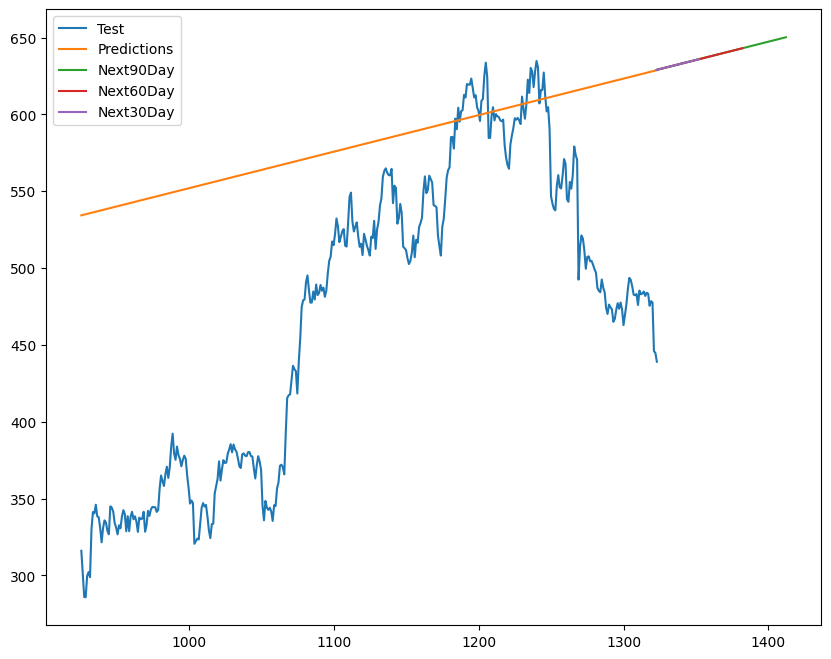
\includegraphics[width=\linewidth]{Linear Plot/ADBE_Linear Regression_7_3.png}
        \caption{ADBE 7-3}
        \label{fig:adbe-7-3}
    \end{subfigure}%
    \hfill
    \begin{subfigure}{0.33\linewidth}
        \centering
        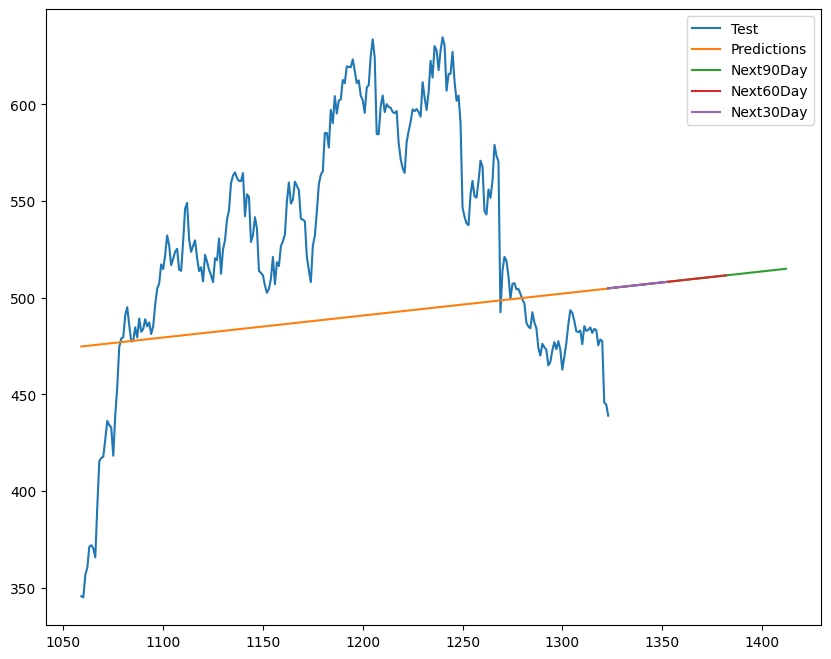
\includegraphics[width=\linewidth]{Linear Plot/ADBE_Linear Regression_8_2.png}
        \caption{ADBE 8-2}
        \label{fig:adbe-8-2}
    \end{subfigure}%
    \hfill
    \begin{subfigure}{0.33\linewidth}
        \centering
        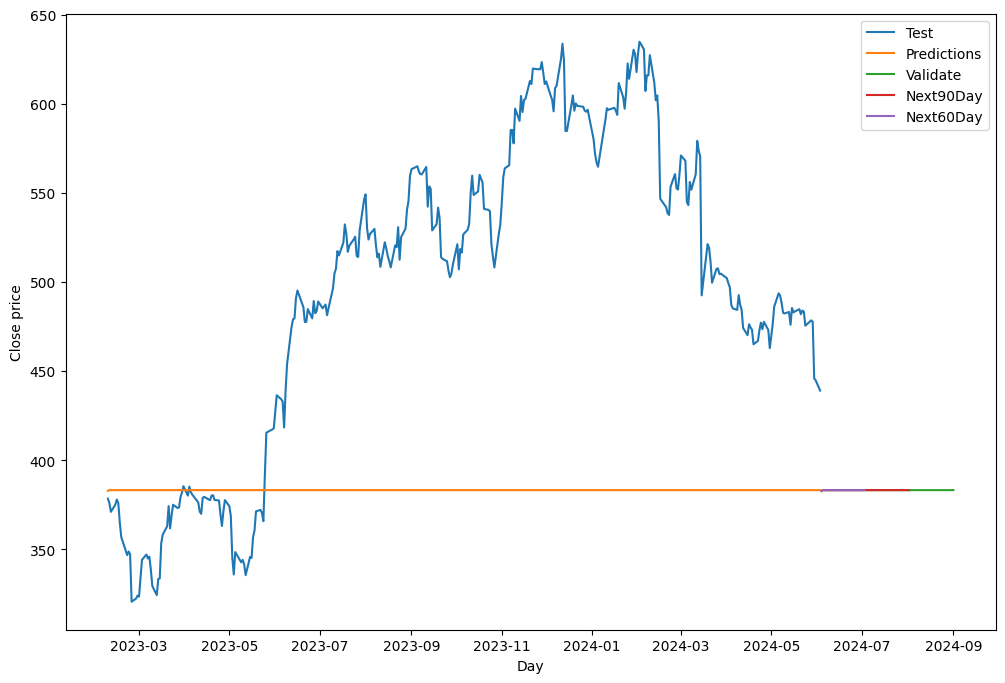
\includegraphics[width=\linewidth]{ARIMA Plot/ARIMA_ADBE_75_25.png}
        \caption{ADBE 75-25}
        \label{fig:adbe-75-25}
    \end{subfigure}
\end{figure}
 \vspace{-20pt}
\begin{figure}[H]
    \centering
    \begin{subfigure}[h]{0.33\linewidth}
        \centering
        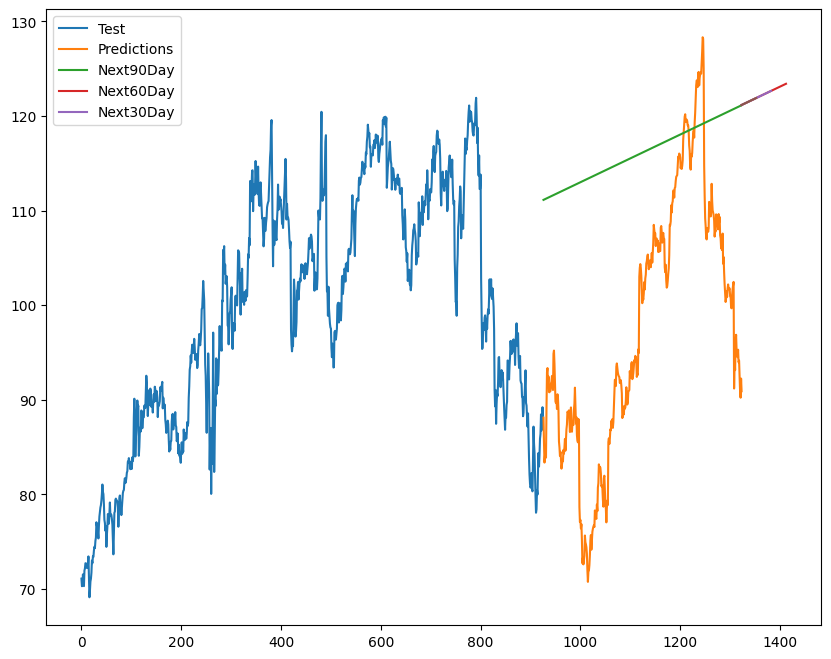
\includegraphics[width=\linewidth]{Linear Plot/AKAM_Linear Regression_7_3.png}
        \caption{AKAM 7-3}
        \label{fig:akam-7-3}
    \end{subfigure}%
    \hfill
    \begin{subfigure}[h]{0.33\linewidth}
        \centering
        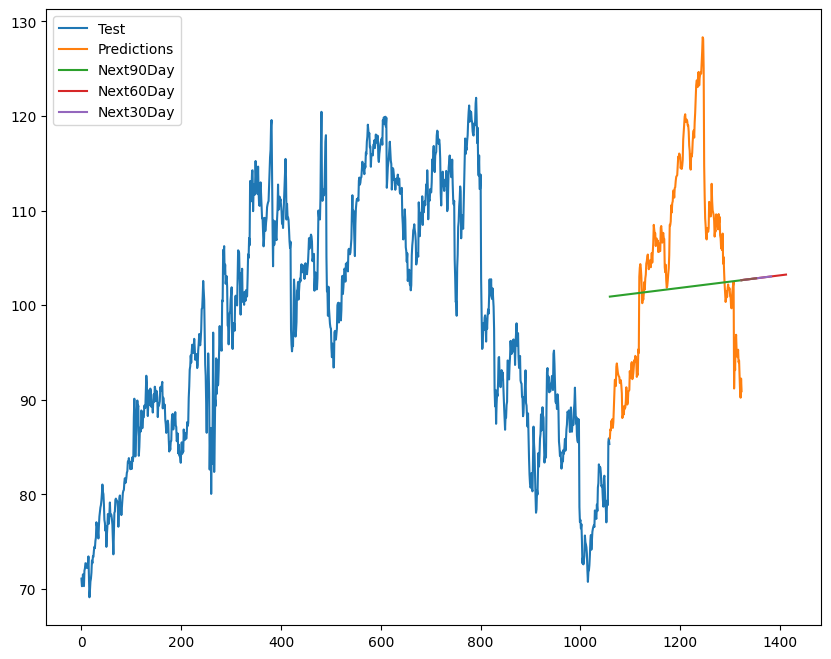
\includegraphics[width=\linewidth]{Linear Plot/AKAM_Linear Regression_8_2.png}
        \caption{AKAM 8-2}
        \label{fig:akam-8-2}
    \end{subfigure}%
    \hfill
    \begin{subfigure}[h]{0.33\linewidth}
        \centering
        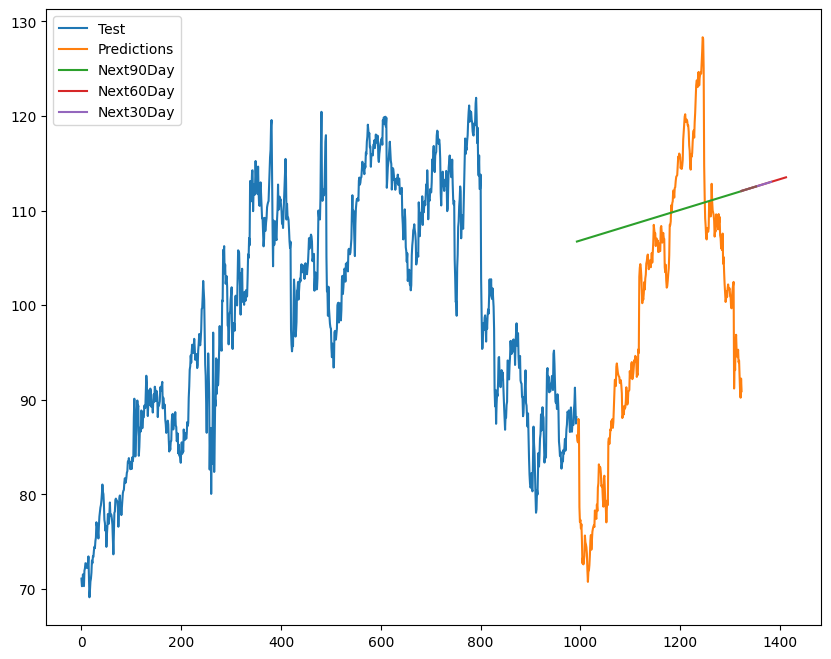
\includegraphics[width=\linewidth]{Linear Plot/AKAM_Linear Regression_75_25.png}
        \caption{AKAM 75-25}
        \label{fig:akam-75-25}
    \end{subfigure}
    \vspace{10pt}
\end{figure}
 \vspace{-20pt}
\begin{figure}[h]
    \centering
    \begin{subfigure}[h]{0.33\linewidth}
        \centering
        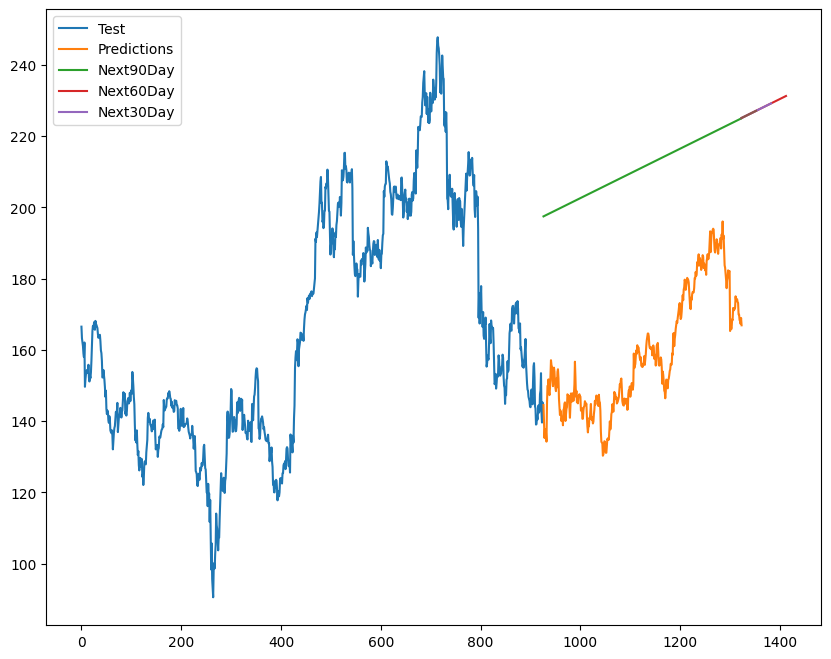
\includegraphics[width=\linewidth]{Linear Plot/FFIV_Linear Regression_7_3.png}
        \caption{FFIV 7-3}
        \label{fig:ffiv-7-3}
    \end{subfigure}%
    \hfill
    \begin{subfigure}[h]{0.33\linewidth}
        \centering
        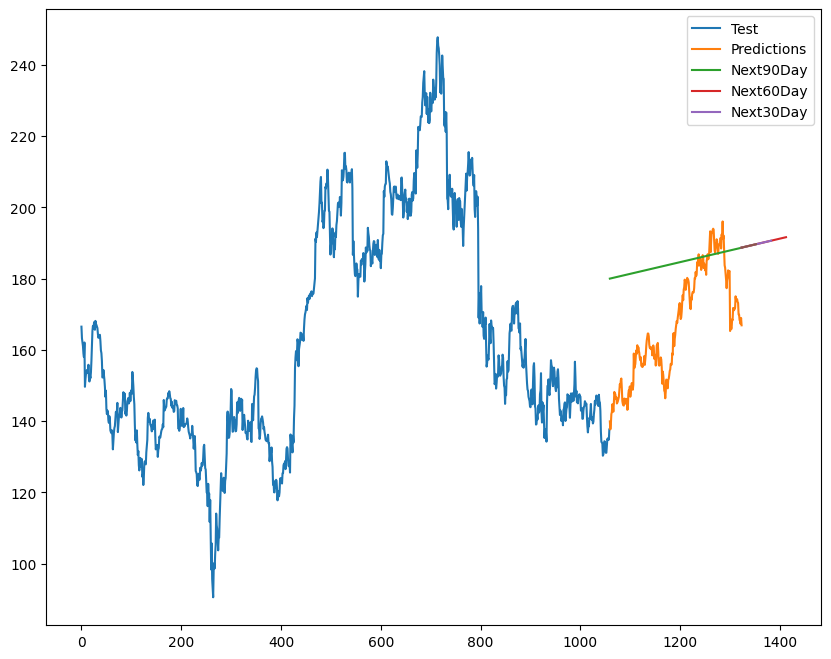
\includegraphics[width=\linewidth]{Linear Plot/FFIV_Linear Regression_8_2.png}
        \caption{FFIV 8-2}
        \label{fig:ffiv-8-2}
    \end{subfigure}%
    \hfill
    \begin{subfigure}[h]{0.33\linewidth}
        \centering
        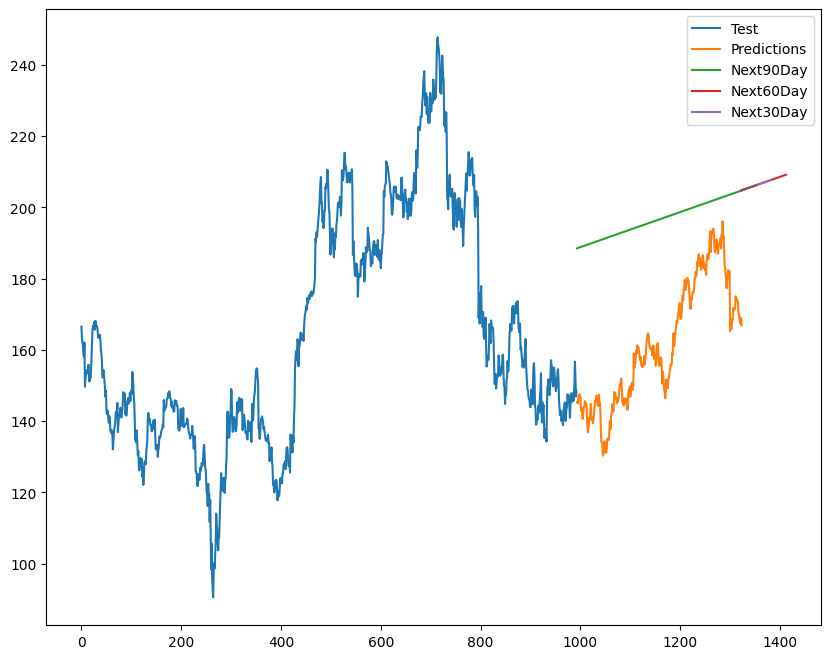
\includegraphics[width=\linewidth]{Linear Plot/FFIV_Linear Regression_75_25.png}
        \caption{FFIV 75-25}
        \label{fig:ffiv-75-25}
    \end{subfigure}
\end{figure}
\vspace{-10pt}
\subsubsection{ARIMA}
\begin{figure}[H]
    \centering
    \begin{subfigure}[h]{0.33\linewidth}
        \centering
        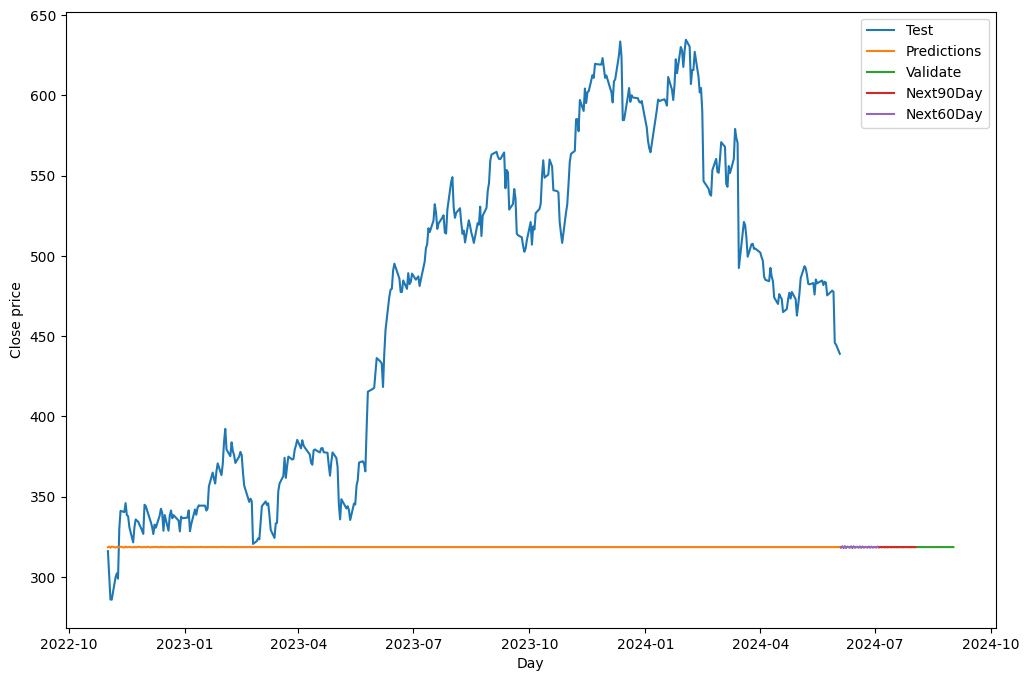
\includegraphics[width=\linewidth]{ARIMA Plot/ARIMA_ADBE_7_3.png}
        \caption{ADBE 7-3}
        \label{fig:adbe-7-3}
    \end{subfigure}%
    \hfill
    \begin{subfigure}[h]{0.33\linewidth}
        \centering
        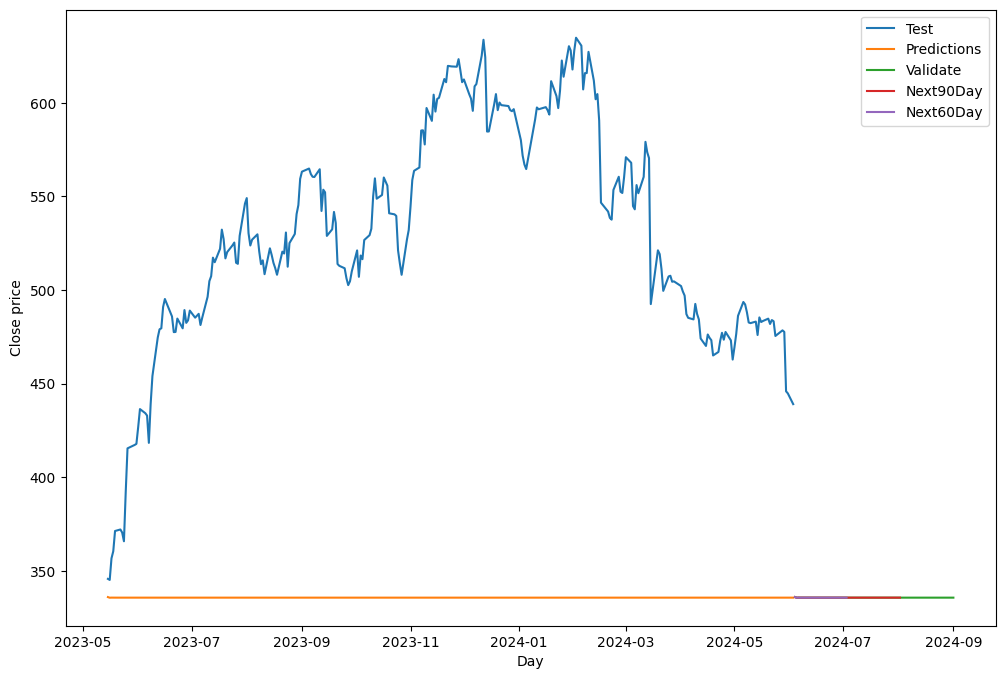
\includegraphics[width=\linewidth]{ARIMA Plot/ARIMA_ADBE_8_2.png}
        \caption{ADBE 8-2}
        \label{fig:adbe-8-2}
    \end{subfigure}%
    \hfill
    \begin{subfigure}[h]{0.33\linewidth}
        \centering
        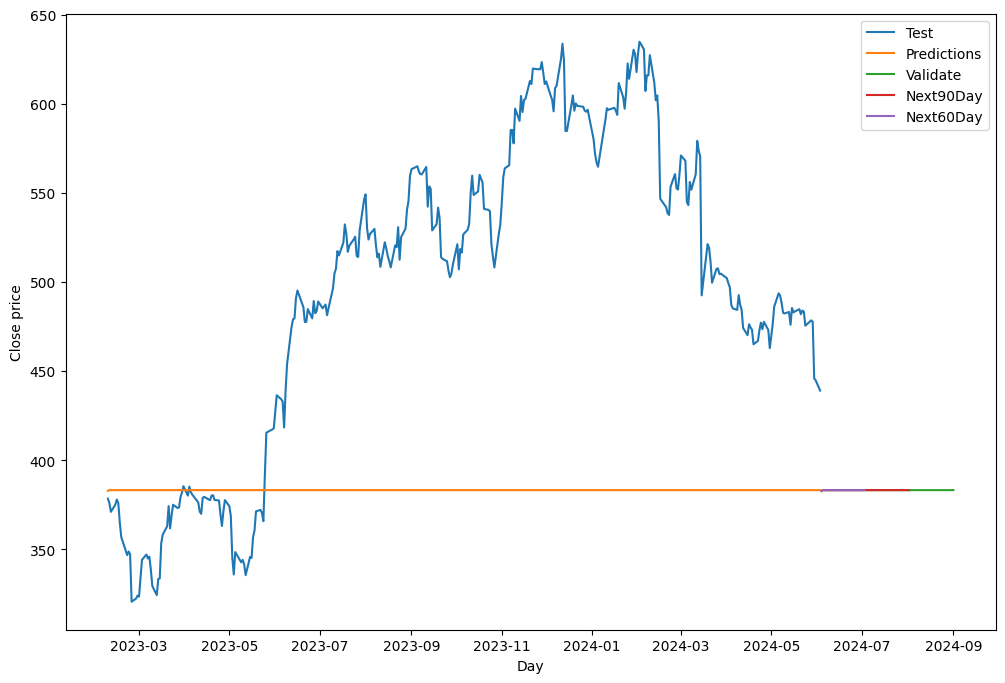
\includegraphics[width=\linewidth]{ARIMA Plot/ARIMA_ADBE_75_25.png}
        \caption{ADBE 75-25}
        \label{fig:adbe-75-25}
    \end{subfigure}
\end{figure}
 \vspace{-20pt}
\begin{figure}[H]
    \centering
    \begin{subfigure}[h]{0.33\linewidth}
        \centering
        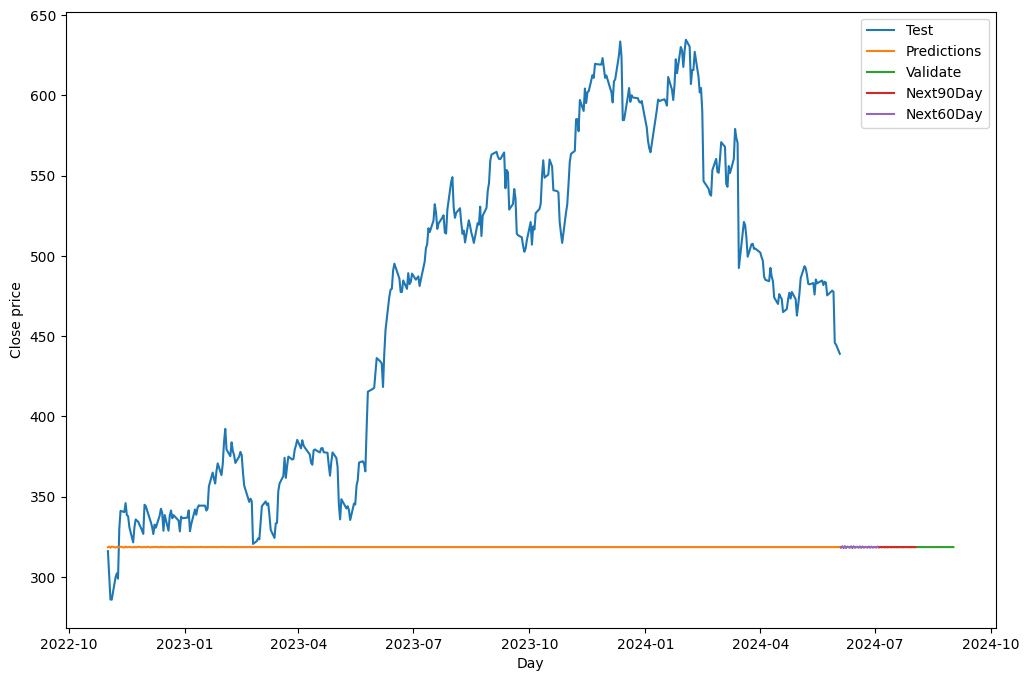
\includegraphics[width=\linewidth]{ARIMA Plot/ARIMA_AKAM_7_3.png}
        \caption{AKAM 7-3}
        \label{fig:akam-7-3}
    \end{subfigure}%
    \hfill
    \begin{subfigure}[h]{0.33\linewidth}
        \centering
        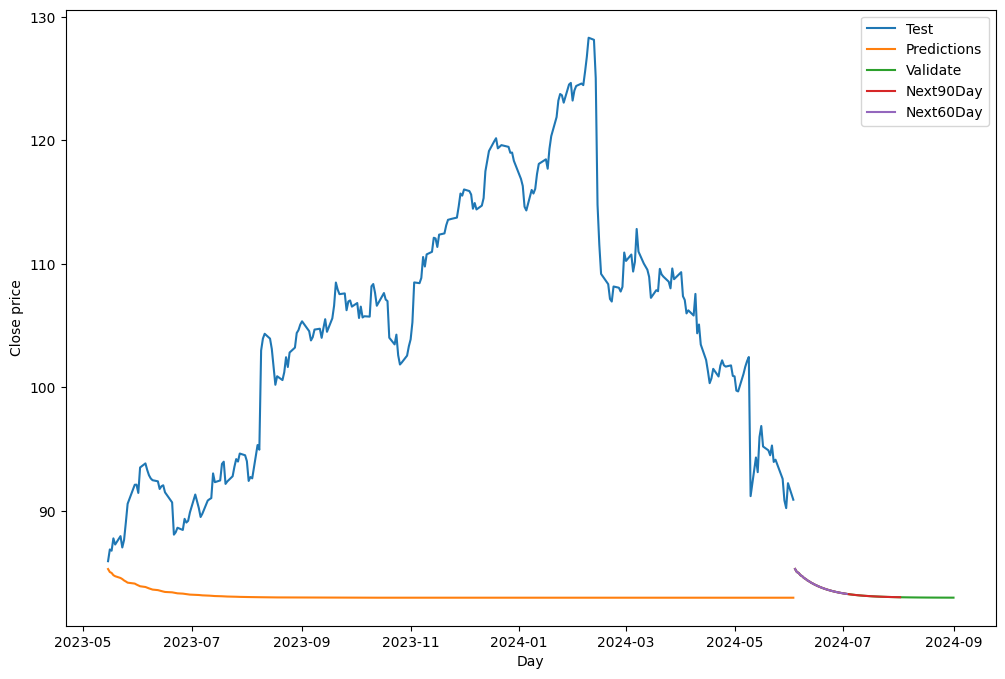
\includegraphics[width=\linewidth]{ARIMA Plot/ARIMA_AKAM_8_2.png}
        \caption{AKAM 8-2}
        \label{fig:akam-8-2}
    \end{subfigure}%
    \hfill
    \begin{subfigure}[h]{0.33\linewidth}
        \centering
        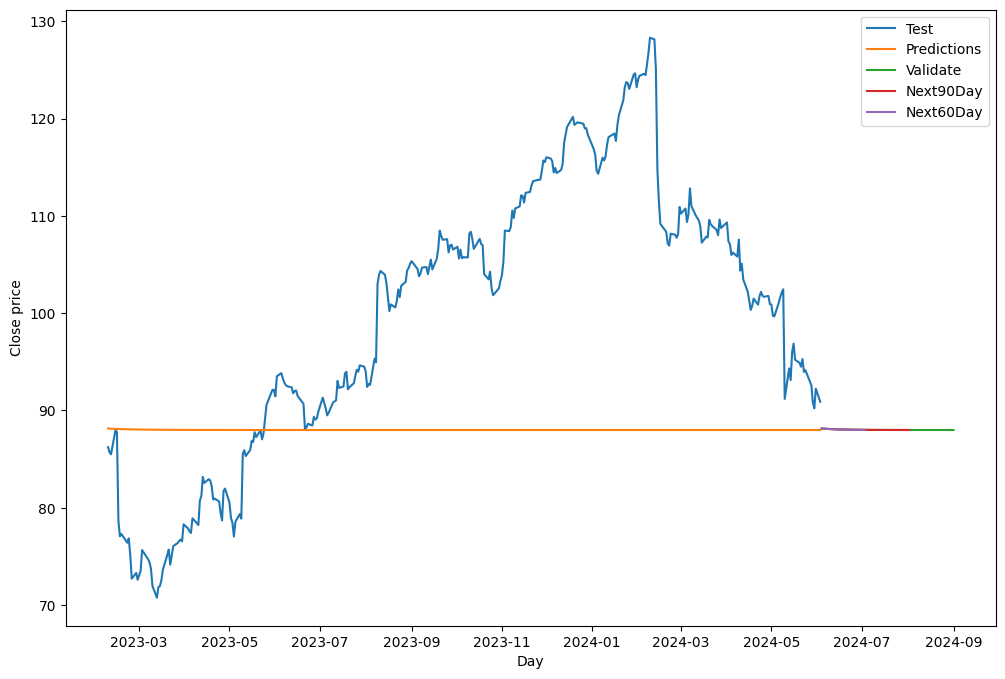
\includegraphics[width=\linewidth]{ARIMA Plot/ARIMA_AKAM_75_25.png}
        \caption{AKAM 75-25}
        \label{fig:akam-75-25}
    \end{subfigure}
\end{figure}
 \vspace{-20pt}
\begin{figure}[H]
    \centering
    \begin{subfigure}[h]{0.33\linewidth}
        \centering
        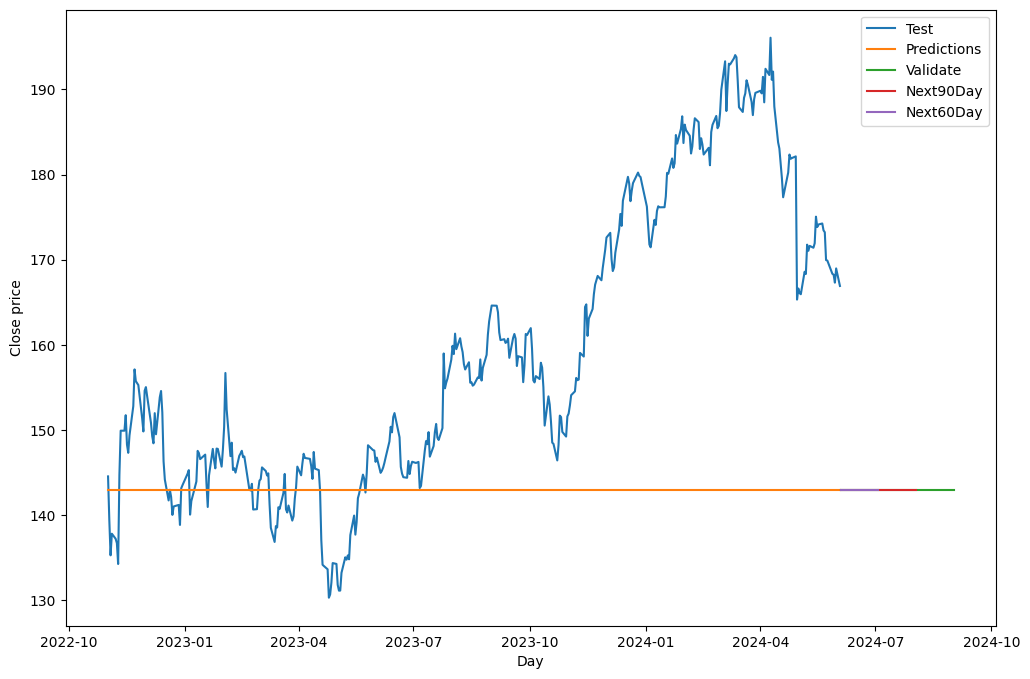
\includegraphics[width=\linewidth]{ARIMA Plot/ARIMA_FFIV_7_3.png}
        \caption{FFIV 7-3}
        \label{fig:ffiv-7-3}
    \end{subfigure}%
    \hfill
    \begin{subfigure}[h]{0.33\linewidth}
        \centering
        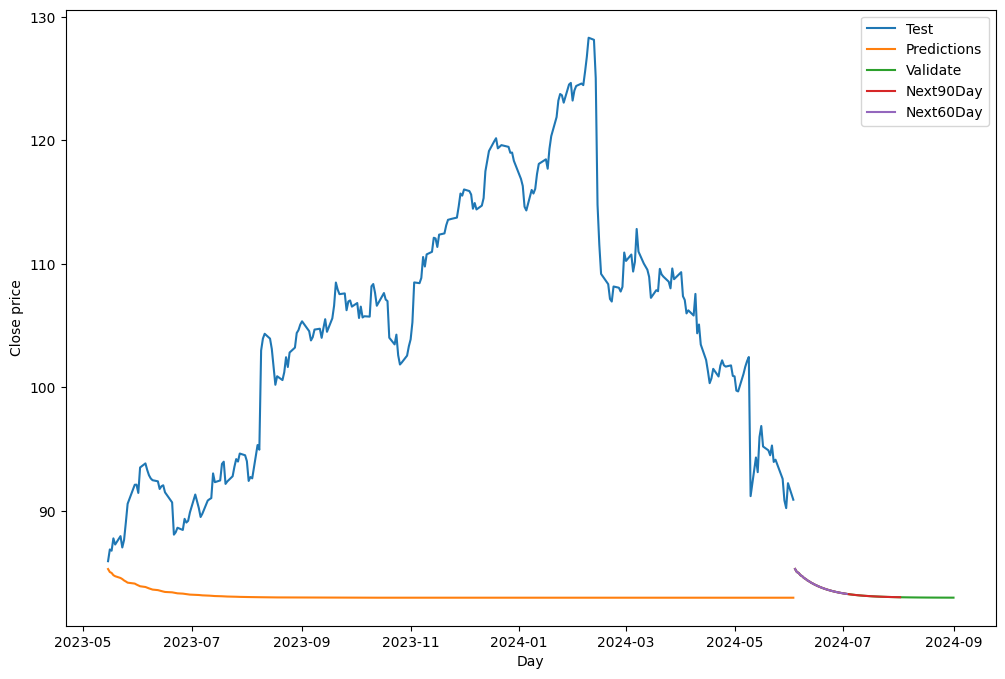
\includegraphics[width=\linewidth]{ARIMA Plot/ARIMA_FFIV_8_2.png}
        \caption{FFIV 8-2}
        \label{fig:ffiv-8-2}
    \end{subfigure}%
    \hfill
    \begin{subfigure}[h]{0.33\linewidth}
        \centering
        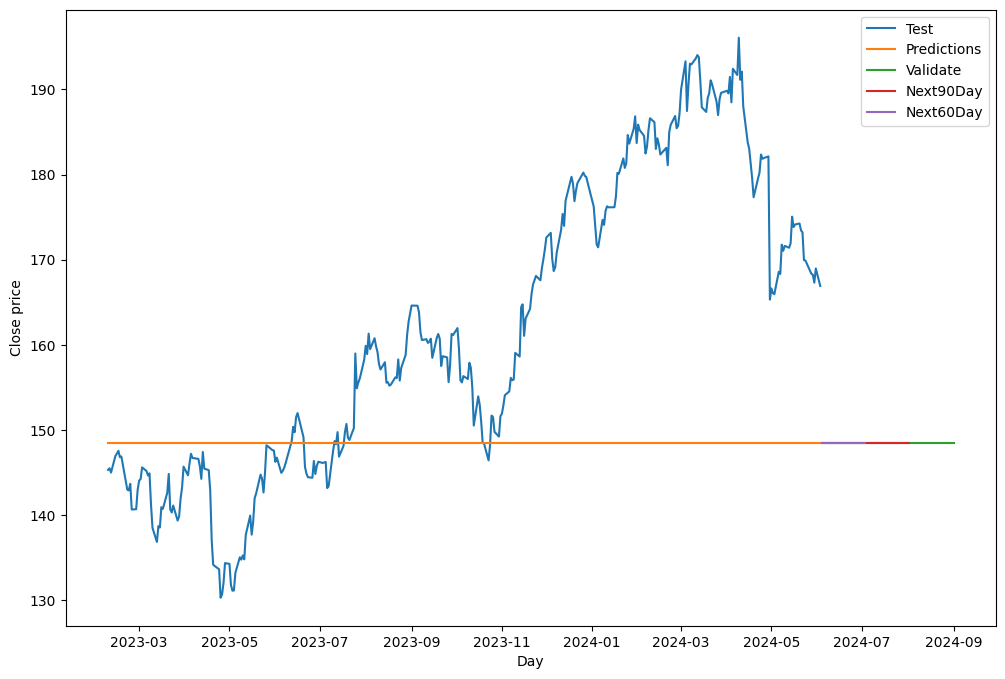
\includegraphics[width=\linewidth]{ARIMA Plot/ARIMA_FFIV_75_25.png}
        \caption{FFIV 75-25}
        \label{fig:ffiv-75-25}
    \end{subfigure}
\end{figure}

\subsubsection{RNN}
\begin{figure}[H]
    \centering
    \begin{subfigure}[h]{0.33\linewidth}
        \centering
        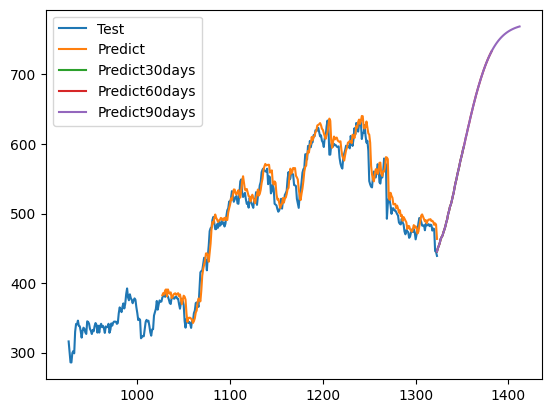
\includegraphics[width=\linewidth]{RNN Plot/RNN_ADBE_7_3.png}
        \caption{ADBE 7-3}
        \label{fig:adbe-7-3}
    \end{subfigure}%
    \hfill
    \begin{subfigure}[h]{0.33\linewidth}
        \centering
        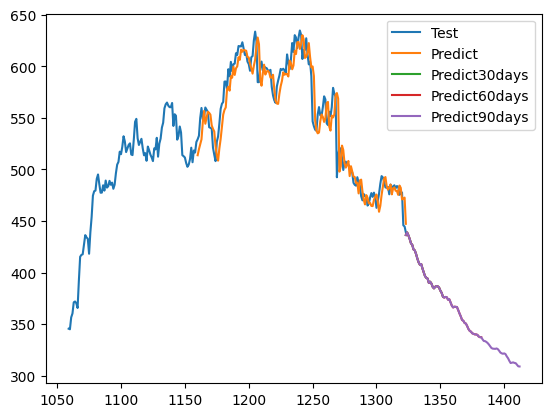
\includegraphics[width=\linewidth]{RNN Plot/RNN_ADBE_8_2.png}
        \caption{ADBE 8-2}
        \label{fig:adbe-8-2}
    \end{subfigure}%
    \hfill
    \begin{subfigure}[h]{0.33\linewidth}
        \centering
        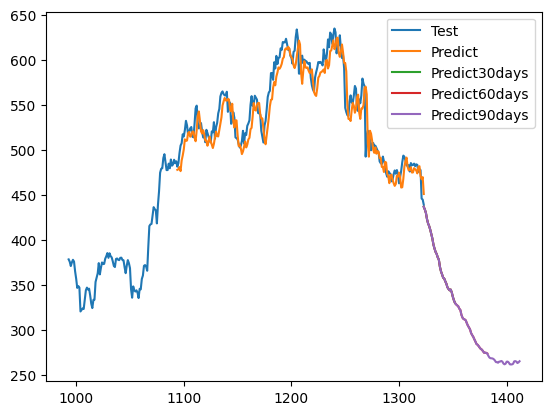
\includegraphics[width=\linewidth]{RNN Plot/RNN_ADBE_75_25.png}
        \caption{ADBE 75-25}
        \label{fig:adbe-75-25}
    \end{subfigure}
    \vspace{10pt}
\end{figure}
 \vspace{-20pt}
\begin{figure}[H]
    \centering
    \begin{subfigure}[h]{0.33\linewidth}
        \centering
        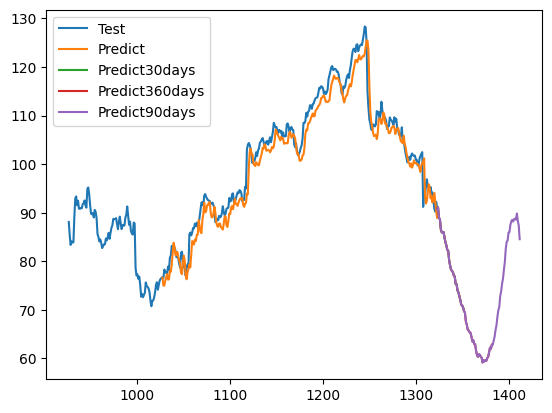
\includegraphics[width=\linewidth]{RNN Plot/RNN_AKAM_7_3.png}
        \caption{AKAM 7-3}
        \label{fig:akam-7-3}
    \end{subfigure}%
    \hfill
    \begin{subfigure}[h]{0.33\linewidth}
        \centering
        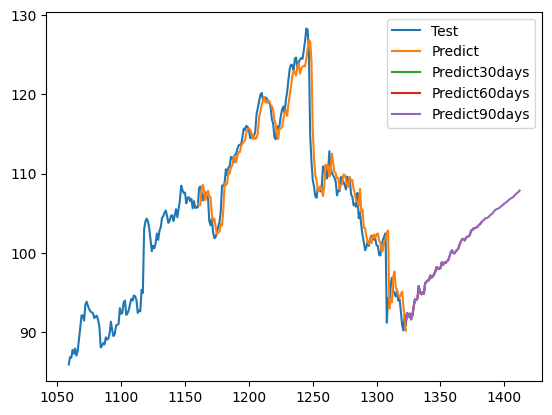
\includegraphics[width=\linewidth]{RNN Plot/RNN_AKAM_8_2.png}
        \caption{AKAM 8-2}
        \label{fig:akam-8-2}
    \end{subfigure}%
    \hfill
    \begin{subfigure}[h]{0.33\linewidth}
        \centering
        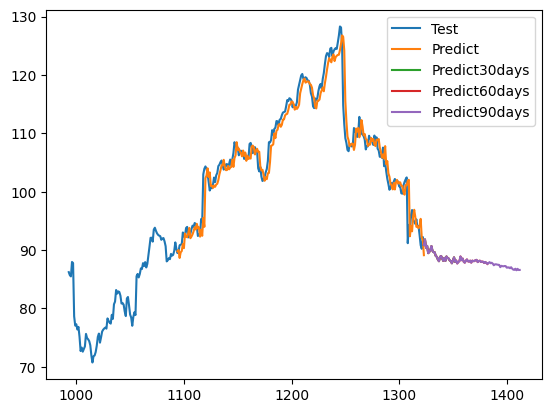
\includegraphics[width=\linewidth]{RNN Plot/RNN_AKAM_75_25.png}
        \caption{AKAM 75-25}
        \label{fig:akam-75-25}
    \end{subfigure}
    \vspace{10pt}
\end{figure}
 \vspace{-20pt}
\begin{figure}[H]
    \centering
    \begin{subfigure}[h]{0.33\linewidth}
        \centering
        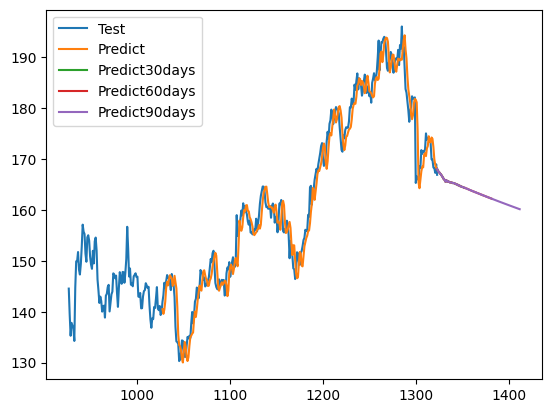
\includegraphics[width=\linewidth]{RNN Plot/RNN_FFIV_7_3.png}
        \caption{FFIV 7-3}
        \label{fig:ffiv-7-3}
    \end{subfigure}%
    \hfill
    \begin{subfigure}[h]{0.33\linewidth}
        \centering
        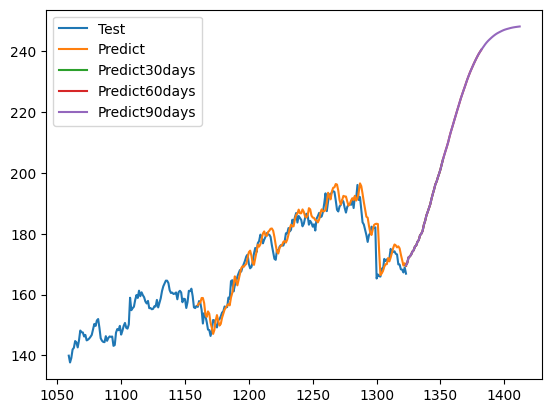
\includegraphics[width=\linewidth]{RNN Plot/RNN_FFIV_8_2.png}
        \caption{FFIV 8-2}
        \label{fig:ffiv-8-2}
    \end{subfigure}%
    \hfill
    \begin{subfigure}[h]{0.33\linewidth}
        \centering
        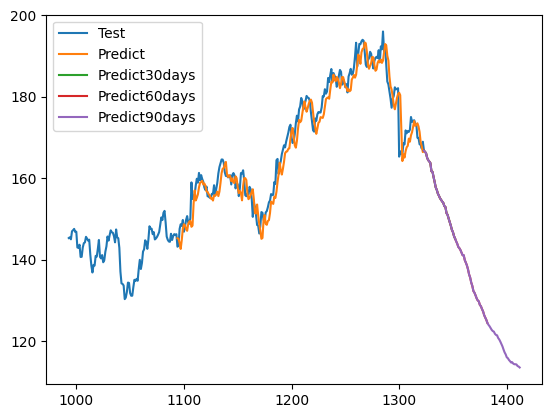
\includegraphics[width=\linewidth]{RNN Plot/RNN_FFIV_75_25.png}
        \caption{FFIV 75-25}
        \label{fig:ffiv-75-25}
    \end{subfigure}
    \vspace{10pt}
\end{figure}

\subsubsection{LSTM}
\begin{figure}[H]
    \centering
    \begin{subfigure}[h]{0.33\linewidth}
        \centering
        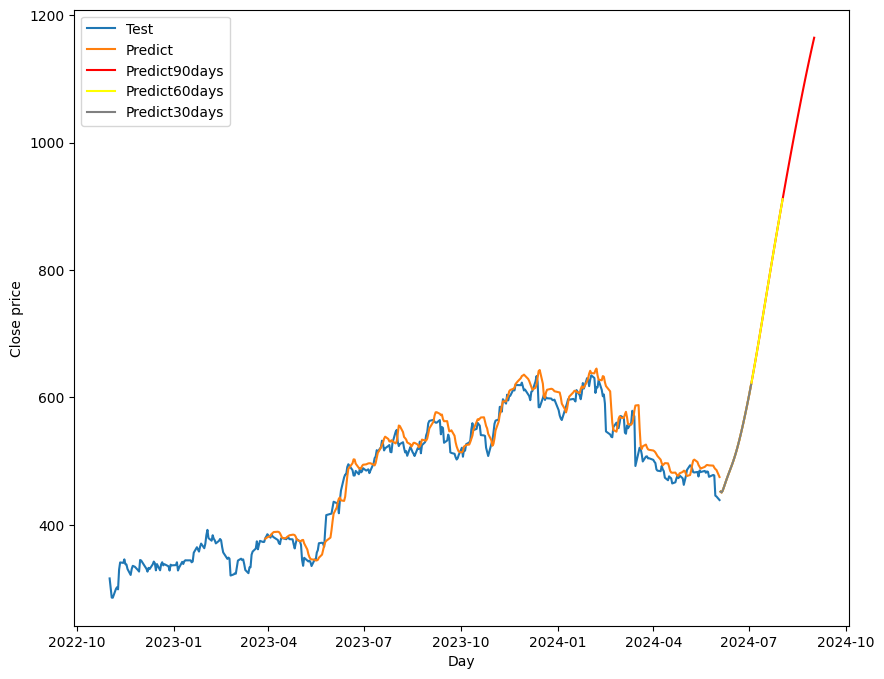
\includegraphics[width=\linewidth]{LSTM Plot/ADBE_LSTM_7_3.png}
        \caption{ADBE 7-3}
        \label{fig:adbe-7-3}
    \end{subfigure}%
    \hfill
    \begin{subfigure}[h]{0.33\linewidth}
        \centering
        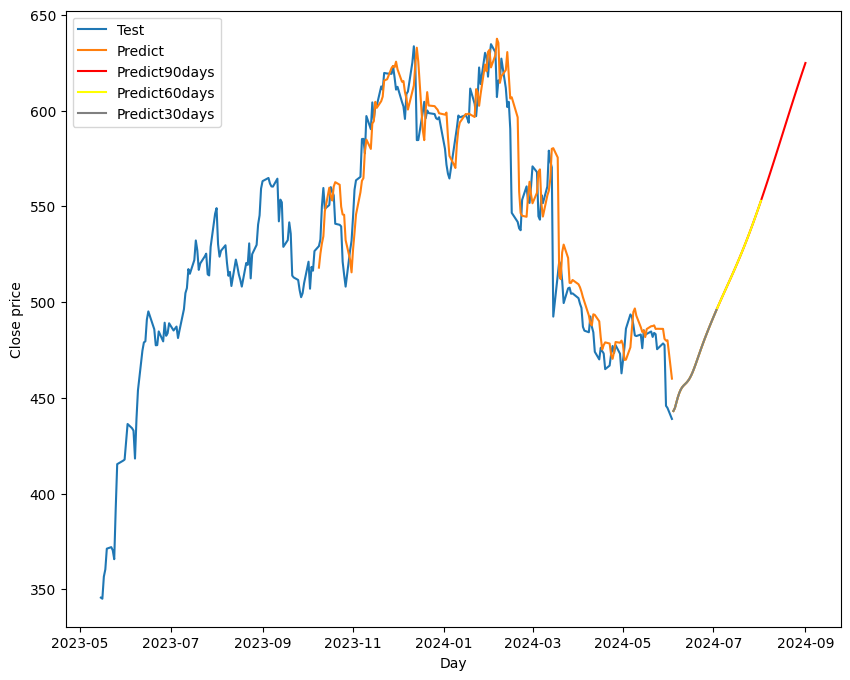
\includegraphics[width=\linewidth]{LSTM Plot/ADBE_LSTM_8_2.png}
        \caption{ADBE 8-2}
        \label{fig:adbe-8-2}
    \end{subfigure}%
    \hfill
    \begin{subfigure}[h]{0.33\linewidth}
        \centering
        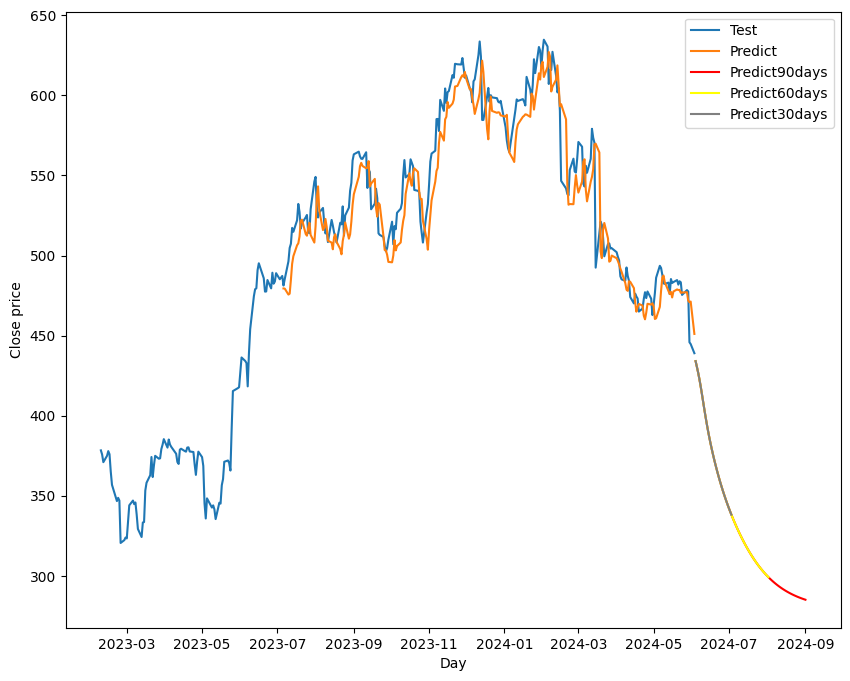
\includegraphics[width=\linewidth]{LSTM Plot/ADBE_LSTM_75_25.png}
        \caption{ADBE 75-25}
        \label{fig:adbe-75-25}
    \end{subfigure}
\end{figure}
 \vspace{-20pt}
\begin{figure}[H]
    \centering
    \begin{subfigure}[b]{0.33\linewidth}
        \centering
        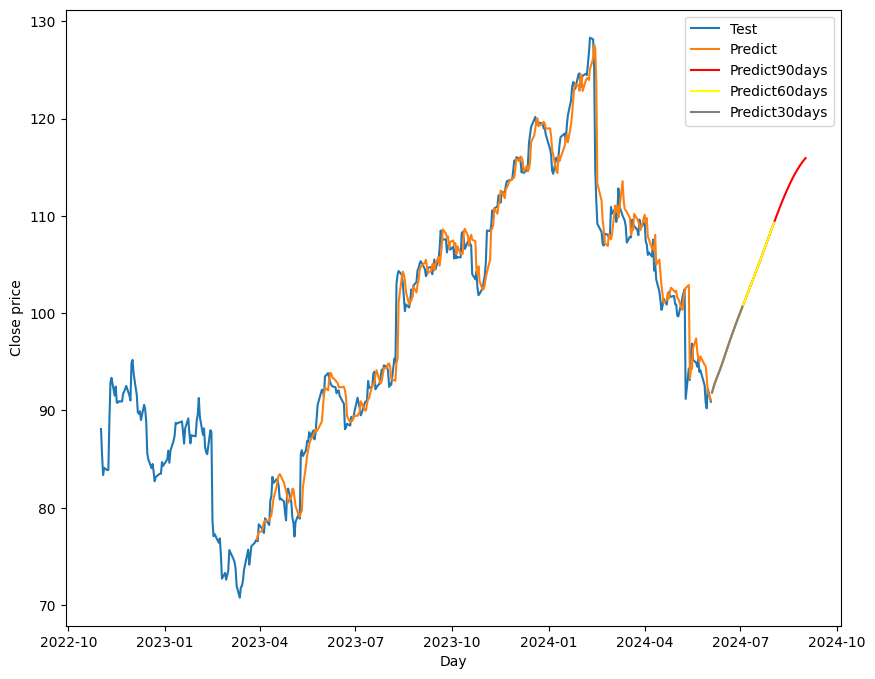
\includegraphics[width=\linewidth]{LSTM Plot/AKAM_LSTM_7_3.png}
        \caption{AKAM 7-3}
        \label{fig:akam-7-3}
    \end{subfigure}%
    \hfill
    \begin{subfigure}[b]{0.33\linewidth}
        \centering
        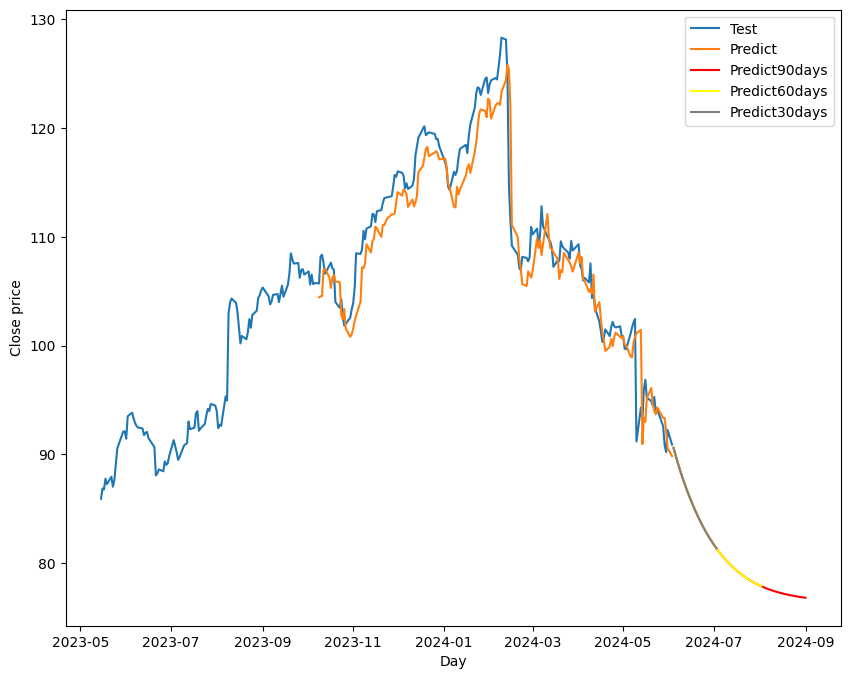
\includegraphics[width=\linewidth]{LSTM Plot/AKAM_LSTM_8_2.png}
        \caption{AKAM 8-2}
        \label{fig:akam-8-2}
    \end{subfigure}%
    \hfill
    \begin{subfigure}[b]{0.33\linewidth}
        \centering
        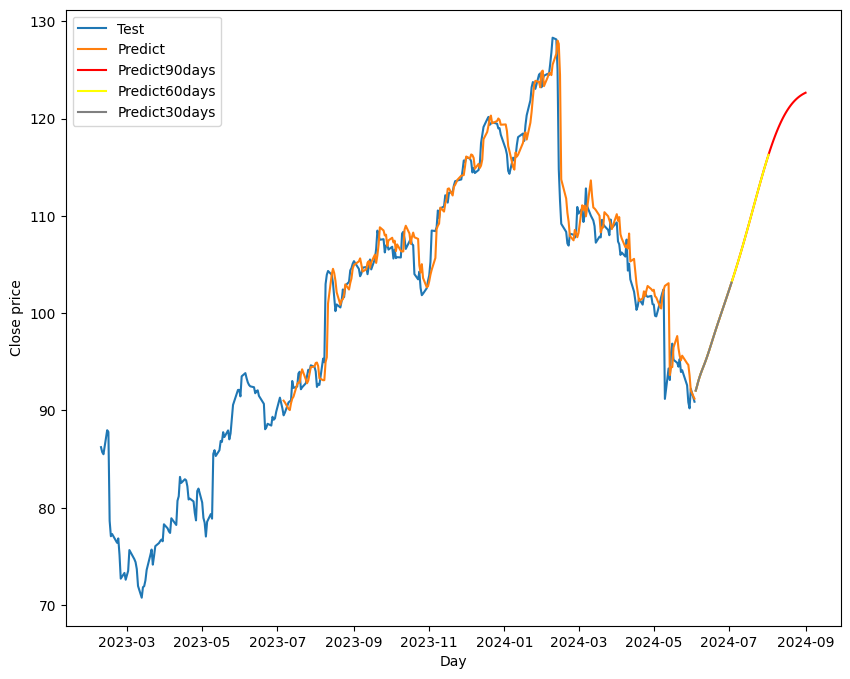
\includegraphics[width=\linewidth]{LSTM Plot/AKAM_LSTM_75_25.png}
        \caption{AKAM 75-25}
        \label{fig:akam-75-25}
    \end{subfigure}
\end{figure}
 \vspace{-20pt}
\begin{figure}[H]
    \centering
    \begin{subfigure}[b]{0.33\linewidth}
        \centering
        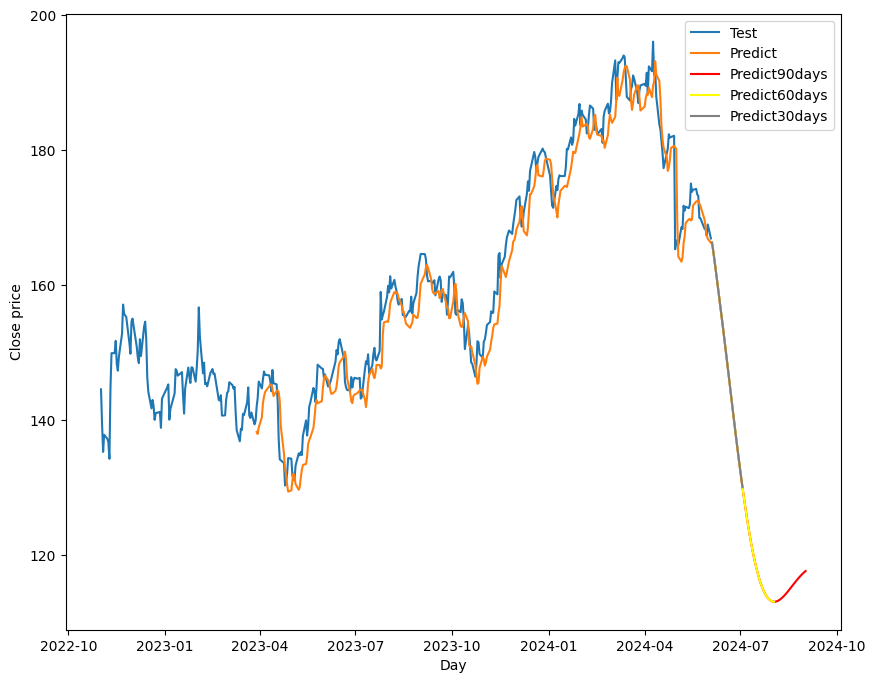
\includegraphics[width=\linewidth]{LSTM Plot/FFIV_LSTM_7_3.png}
        \caption{FFIV 7-3}
        \label{fig:ffiv-7-3}
    \end{subfigure}%
    \hfill
    \begin{subfigure}[b]{0.33\linewidth}
        \centering
        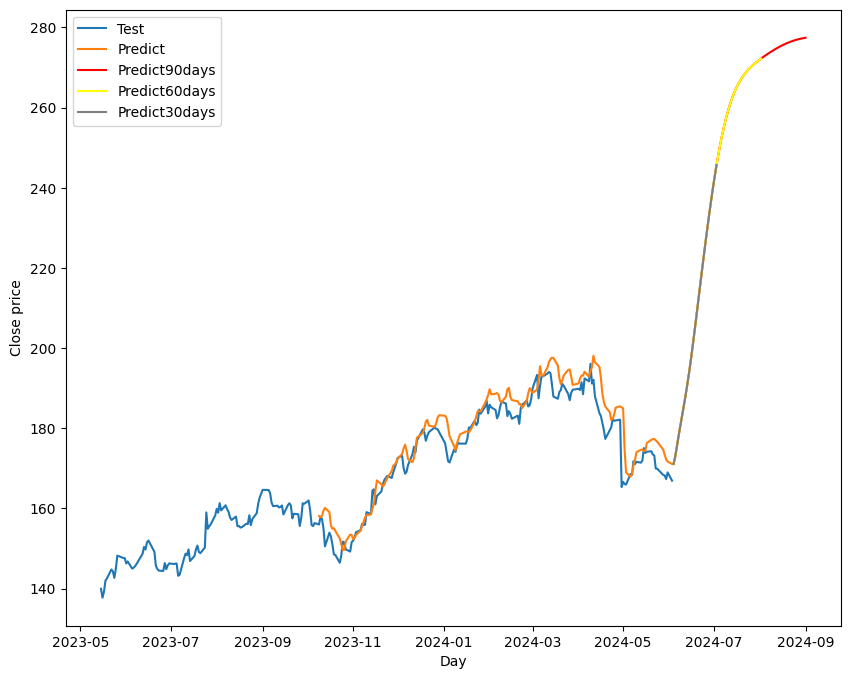
\includegraphics[width=\linewidth]{LSTM Plot/FFIV_LSTM_8_2.png}
        \caption{FFIV 8-2}
        \label{fig:ffiv-8-2}
    \end{subfigure}%
    \hfill
    \begin{subfigure}[b]{0.33\linewidth}
        \centering
        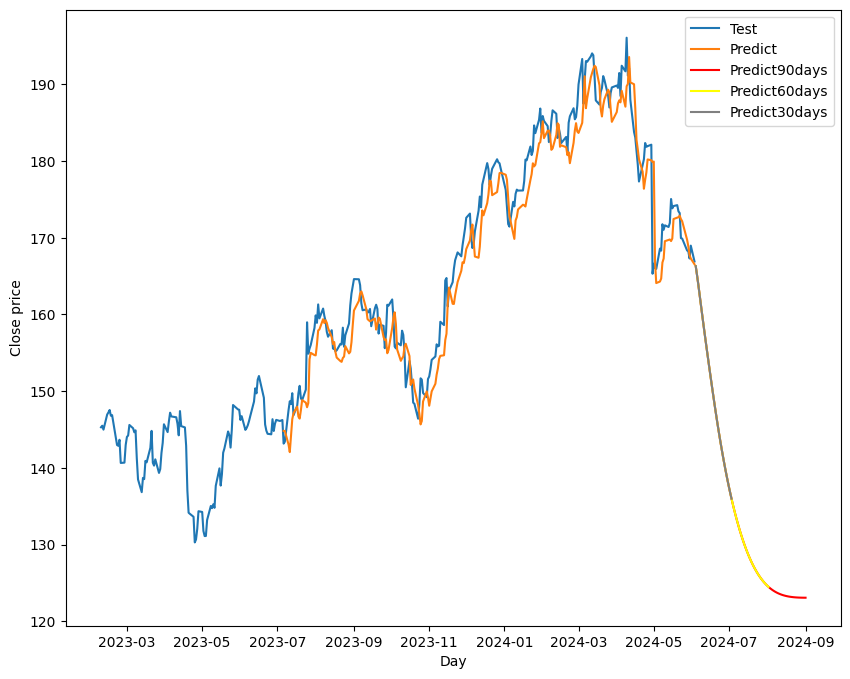
\includegraphics[width=\linewidth]{LSTM Plot/FFIV_LSTM_75_25.png}
        \caption{FFIV 75-25}
        \label{fig:ffiv-75-25}
    \end{subfigure}
    \vspace{10pt}
\end{figure}
\subsubsection{GRU}
\begin{figure}[H]
    \centering
    \begin{subfigure}[b]{0.33\linewidth}
        \centering
        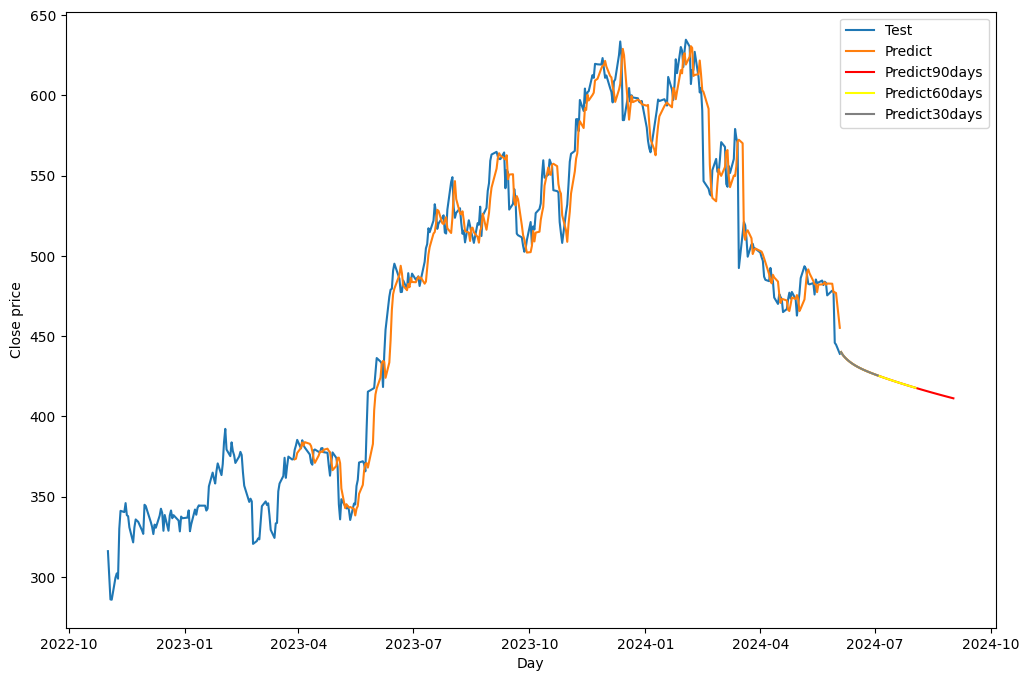
\includegraphics[width=\linewidth]{GRU Plot/GRU_ADBE_7_3.png}
        \caption{ADBE 7-3}
        \label{fig:adbe-7-3}
    \end{subfigure}%
    \hfill
    \begin{subfigure}[b]{0.33\linewidth}
        \centering
        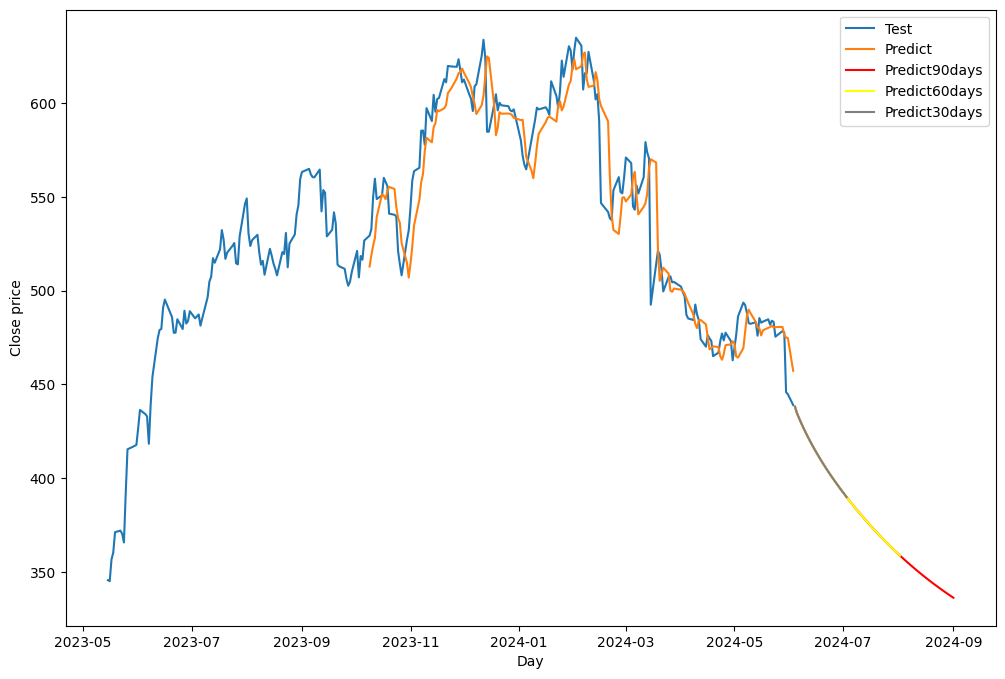
\includegraphics[width=\linewidth]{GRU Plot/GRU_ADBE_8_2.png}
        \caption{ADBE 8-2}
        \label{fig:adbe-8-2}
    \end{subfigure}%
    \hfill
    \begin{subfigure}[b]{0.33\linewidth}
        \centering
        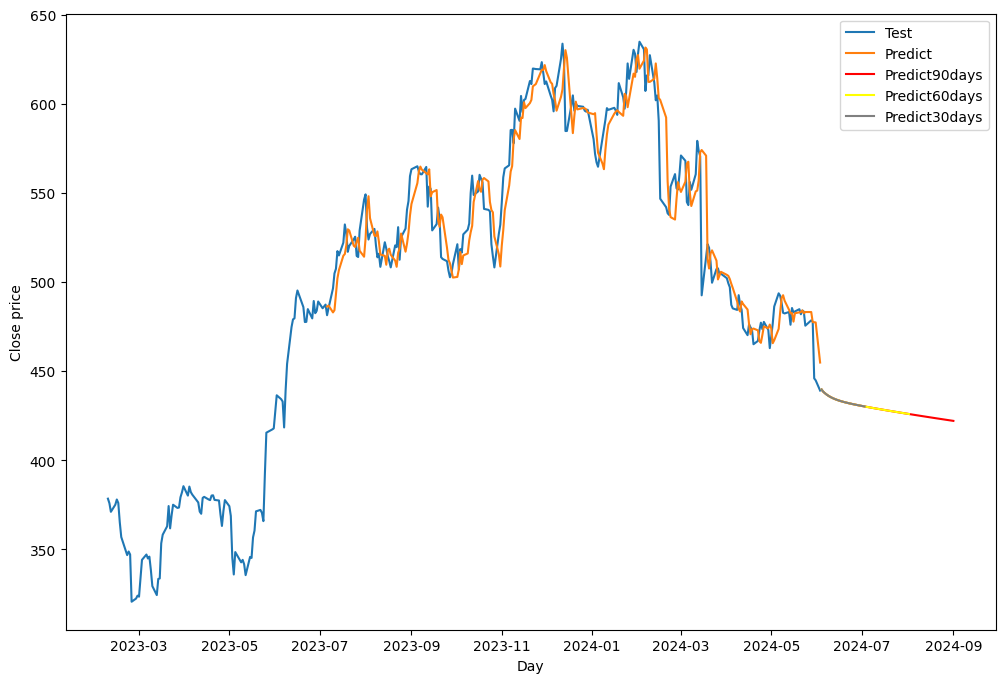
\includegraphics[width=\linewidth]{GRU Plot/GRU_ADBE_75_25.png}
        \caption{ADBE 75-25}
        \label{fig:adbe-75-25}
    \end{subfigure}
    \vspace{10pt}
\end{figure}
 \vspace{-20pt}
\begin{figure}[H]
    \centering
    \begin{subfigure}[b]{0.33\linewidth}
        \centering
        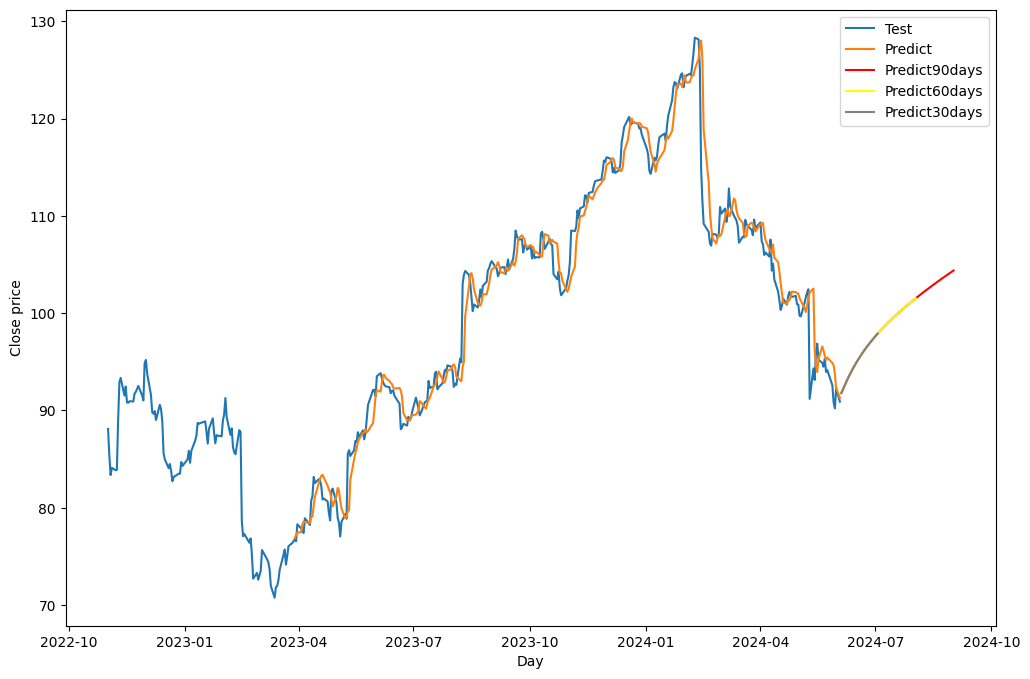
\includegraphics[width=\linewidth]{GRU Plot/GRU_AKAM_7_3.png}
        \caption{AKAM 7-3}
        \label{fig:akam-7-3}
    \end{subfigure}%
    \hfill
    \begin{subfigure}[b]{0.33\linewidth}
        \centering
        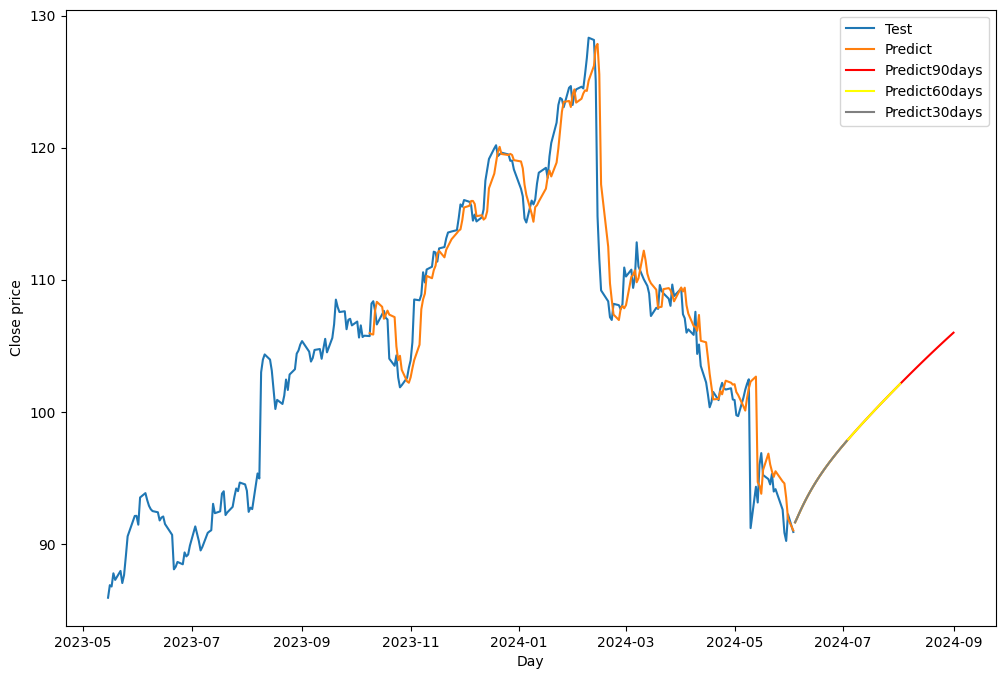
\includegraphics[width=\linewidth]{GRU Plot/GRU_AKAM_8_2.png}
        \caption{AKAM 8-2}
        \label{fig:akam-8-2}
    \end{subfigure}%
    \hfill
    \begin{subfigure}[b]{0.33\linewidth}
        \centering
        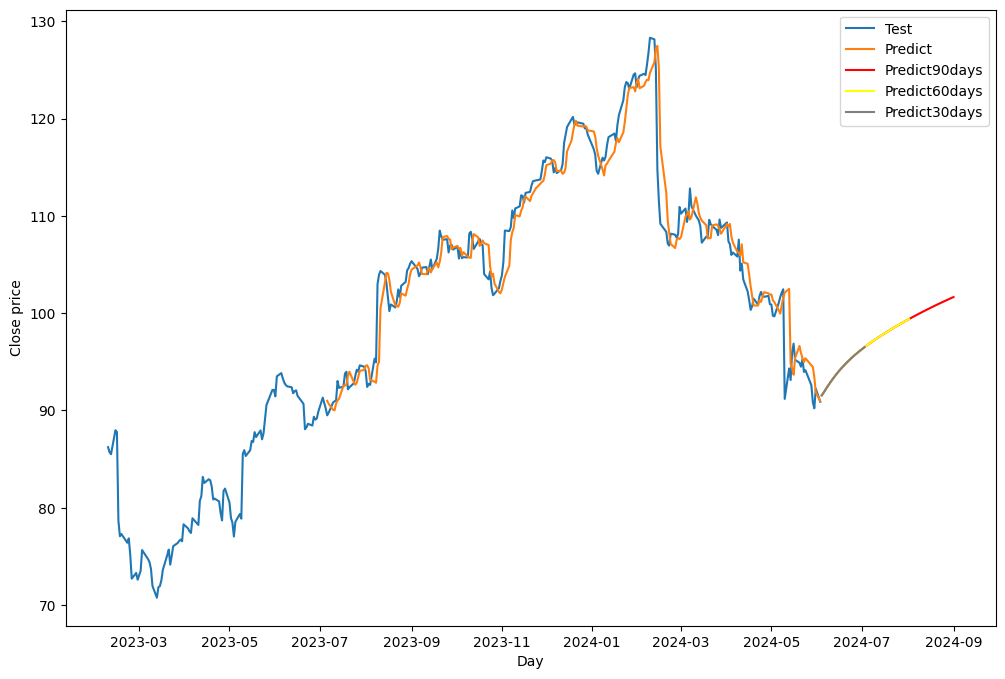
\includegraphics[width=\linewidth]{GRU Plot/GRU_AKAM_75_25.png}
        \caption{AKAM 75-25}
        \label{fig:akam-75-25}
    \end{subfigure}
    \vspace{10pt}
\end{figure}
 \vspace{-20pt}
\begin{figure}[H]
    \centering
    \begin{subfigure}[b]{0.33\linewidth}
        \centering
        \includegraphics[width=\linewidth]{GRU Plot/GRU_FFIV_7_3.png}
        \caption{FFIV 7-3}
        \label{fig:ffiv-7-3}
    \end{subfigure}%
    \hfill
    \begin{subfigure}[b]{0.33\linewidth}
        \centering
        \includegraphics[width=\linewidth]{GRU Plot/GRU_FFIV_8_2.png}
        \caption{FFIV 8-2}
        \label{fig:ffiv-8-2}
    \end{subfigure}%
    \hfill
    \begin{subfigure}[b]{0.33\linewidth}
        \centering
        \includegraphics[width=\linewidth]{GRU Plot/GRU_FFIV_75_25.png}
        \caption{FFIV 75-25}
        \label{fig:ffiv-75-25}
    \end{subfigure}
\end{figure}
\subsubsection{ETS}
\begin{figure}[H]
    \centering
    \begin{subfigure}[b]{0.33\linewidth}
        \centering
        \includegraphics[width=\linewidth]{ETS Plot/ADBE_ETS_7_3.png}
        \caption{ADBE 7-3}
        \label{fig:adbe-7-3}
    \end{subfigure}%
    \hfill
    \begin{subfigure}[b]{0.33\linewidth}
        \centering
        \includegraphics[width=\linewidth]{ETS Plot/ADBE_ETS_8_2.png}
        \caption{ADBE 8-2}
        \label{fig:adbe-8-2}
    \end{subfigure}%
    \hfill
    \begin{subfigure}[b]{0.33\linewidth}
        \centering
        \includegraphics[width=\linewidth]{ETS Plot/ADBE_ETS_75_25.png}
        \caption{ADBE 75-25}
        \label{fig:adbe-75-25}
    \end{subfigure}
\end{figure}
 \vspace{-10pt}
\begin{figure}[H]
    \centering
    \begin{subfigure}[b]{0.33\linewidth}
        \centering
        \includegraphics[width=\linewidth]{ETS Plot/AKAM_ETS_7_3.png}
        \caption{AKAM 7-3}
        \label{fig:akam-7-3}
    \end{subfigure}%
    \hfill
    \begin{subfigure}[b]{0.33\linewidth}
        \centering
        \includegraphics[width=\linewidth]{ETS Plot/AKAM_ETS_8_2.png}
        \caption{AKAM 8-2}
        \label{fig:akam-8-2}
    \end{subfigure}%
    \hfill
    \begin{subfigure}[b]{0.33\linewidth}
        \centering
        \includegraphics[width=\linewidth]{ETS Plot/AKAM_ETS_75_25.png}
        \caption{AKAM 75-25}
        \label{fig:akam-75-25}
    \end{subfigure}
\end{figure}
 \vspace{-10pt}
\begin{figure}[H]
    \centering
    \begin{subfigure}[b]{0.33\linewidth}
        \centering
        \includegraphics[width=\linewidth]{ETS Plot/FFIV_ETS_7_3.png}
        \caption{FFIV 7-3}
        \label{fig:ffiv-7-3}
    \end{subfigure}%
    \hfill
    \begin{subfigure}[b]{0.33\linewidth}
        \centering
        \includegraphics[width=\linewidth]{ETS Plot/FFIV_ETS_8_2.png}
        \caption{FFIV 8-2}
        \label{fig:ffiv-8-2}
    \end{subfigure}%
    \hfill
    \begin{subfigure}[b]{0.33\linewidth}
        \centering
        \includegraphics[width=\linewidth]{ETS Plot/FFIV_ETS_75_25.png}
        \caption{FFIV 75-25}
        \label{fig:ffiv-75-25}
    \end{subfigure}
\end{figure}
\subsubsection{META-LEARNING}
\begin{figure}[H]
    \centering
    \begin{subfigure}[b]{0.33\linewidth}
        \centering
        \includegraphics[width=\linewidth]{Meta-learning Plot/ML_ADBE_7_3.png}
        \caption{ADBE 7-3}
        \label{fig:adbe-7-3}
    \end{subfigure}%
    \hfill
    \begin{subfigure}[b]{0.33\linewidth}
        \centering
        \includegraphics[width=\linewidth]{Meta-learning Plot/ML_ADBE_8_2.png}
        \caption{ADBE 8-2}
        \label{fig:adbe-8-2}
    \end{subfigure}%
    \hfill
    \begin{subfigure}[b]{0.33\linewidth}
        \centering
        \includegraphics[width=\linewidth]{Meta-learning Plot/ML_ADBE_75_25.png}
        \caption{ADBE 75-25}
        \label{fig:adbe-75-25}
    \end{subfigure}
\end{figure}
 \vspace{-10pt}
\begin{figure}[H]
    \centering
    \begin{subfigure}[b]{0.33\linewidth}
        \centering
        \includegraphics[width=\linewidth]{Meta-learning Plot/ML_AKAM_7_3.png}
        \caption{AKAM 7-3}
        \label{fig:akam-7-3}
    \end{subfigure}%
    \hfill
    \begin{subfigure}[b]{0.33\linewidth}
        \centering
        \includegraphics[width=\linewidth]{Meta-learning Plot/ML_AKAM_8_2.png}
        \caption{AKAM 8-2}
        \label{fig:akam-8-2}
    \end{subfigure}%
    \hfill
    \begin{subfigure}[b]{0.33\linewidth}
        \centering
        \includegraphics[width=\linewidth]{Meta-learning Plot/ML_AKAM_75_25.png}
        \caption{AKAM 75-25}
        \label{fig:akam-75-25}
    \end{subfigure}
\end{figure}
 \vspace{-10pt}
\begin{figure}[H]
    \centering
    \begin{subfigure}[b]{0.33\linewidth}
        \centering
        \includegraphics[width=\linewidth]{Meta-learning Plot/ML_FFIV_7_3.png}
        \caption{FFIV 7-3}
        \label{fig:ffiv-7-3}
    \end{subfigure}%
    \hfill
    \begin{subfigure}[b]{0.33\linewidth}
        \centering
        \includegraphics[width=\linewidth]{Meta-learning Plot/ML_FFIV_8_2.png}
        \caption{FFIV 8-2}
        \label{fig:ffiv-8-2}
    \end{subfigure}%
    \hfill
    \begin{subfigure}[b]{0.33\linewidth}
        \centering
        \includegraphics[width=\linewidth]{Meta-learning Plot/ML_FFIV_75_25.png}
        \caption{FFIV 75-25}
        \label{fig:ffiv-75-25}
    \end{subfigure}
\end{figure}
\subsubsection{ADDRNN}
\begin{figure}[H]
    \centering
    \begin{subfigure}[b]{0.33\linewidth}
        \centering
        \includegraphics[width=\linewidth]{AddRNN Plot/AddRNN_ADBE_7_3.png}
        \caption{ADBE 7-3}
        \label{fig:adbe-7-3}
    \end{subfigure}%
    \hfill
    \begin{subfigure}[b]{0.33\linewidth}
        \centering
        \includegraphics[width=\linewidth]{AddRNN Plot/AddRNN_ADBE_8_2.png}
        \caption{ADBE 8-2}
        \label{fig:adbe-8-2}
    \end{subfigure}%
    \hfill
    \begin{subfigure}[b]{0.33\linewidth}
        \centering
        \includegraphics[width=\linewidth]{AddRNN Plot/AddRNN_ADBE_75_25.png}
        \caption{ADBE 75-25}
        \label{fig:adbe-75-25}
    \end{subfigure}
\end{figure}
 \vspace{-60pt}
\begin{figure}[htbp]
    \centering
    \begin{subfigure}[b]{0.33\linewidth}
        \centering
        \includegraphics[width=\linewidth]{AddRNN Plot/AddRNN_AKAM_7_3.png}
        \caption{AKAM 7-3}
        \label{fig:akam-7-3}
    \end{subfigure}%
    \hfill
    \begin{subfigure}[b]{0.33\linewidth}
        \centering
        \includegraphics[width=\linewidth]{AddRNN Plot/AddRNN_AKAM_8_2.png}
        \caption{AKAM 8-2}
        \label{fig:akam-8-2}
    \end{subfigure}%
    \hfill
    \begin{subfigure}[b]{0.33\linewidth}
        \centering
        \includegraphics[width=\linewidth]{AddRNN Plot/AddRNN_AKAM_75_25.png}
        \caption{AKAM 75-25}
        \label{fig:akam-75-25}
    \end{subfigure}
\end{figure}
 \vspace{-20pt}
\begin{figure}[H]
    \centering
    \begin{subfigure}[b]{0.33\linewidth}
        \centering
        \includegraphics[width=\linewidth]{AddRNN Plot/AddRNN_FFIV_7_3.png}
        \caption{FFIV 7-3}
        \label{fig:ffiv-7-3}
    \end{subfigure}%
    \hfill
    \begin{subfigure}[b]{0.33\linewidth}
        \centering
        \includegraphics[width=\linewidth]{AddRNN Plot/AddRNN_FFIV_8_2.png}
        \caption{FFIV 8-2}
        \label{fig:ffiv-8-2}
    \end{subfigure}%
    \hfill
    \begin{subfigure}[b]{0.33\linewidth}
        \centering
        \includegraphics[width=\linewidth]{AddRNN Plot/AddRNN_FFIV_75_25.png}
        \caption{FFIV 75-25}
        \label{fig:ffiv-75-25}
    \end{subfigure}
\end{figure}

\subsection{Evaluation models}
\vspace{-20pt}
\begin{table}[H]
\centering
\begin{tabular}{cccccc}
\toprule
\textbf{Model} & \textbf{Train/Test} & \textbf{RMSE} & \textbf{MAPE} & \textbf{MAE} \\ 
\midrule
Linear & 7/3 & 137.51 & 0.29 & 114.72 \\ 
       & 8/2 & 70.70 & 0.11 & 58.60 \\ 
       & 75/25 & 83.15 & 0.16 & 66.51 \\ 
\midrule
LSTM   & 7/3 & 16.51 & 0.02 & 12.51 \\ 
       & 8/2 & 12.81 & 0.02 & 8.84 \\ 
       & 75/25 & 13.45 & 0.02 & 10.51 \\ 
\midrule
ETS    & 7/3 & 176.58 & 0.28 & 146.80 \\ 
       & 8/2 & 210.92 & 0.37 & 199.19 \\ 
       & 75/25 & 103.77 & 0.17 & 85.13 \\ 
\midrule
ARIMA  & 7/3 & 179.88 & 28.95 & 151.05 \\ 
       & 8/2 & 202.66 & 35.66 & 193.51 \\ 
       & 75/25 & 141.94 & 22.91 & 122.58 \\ 
\midrule
GRU    & 7/3 & 11.15 & 1.53 & 7.77 \\ 
       & 8/2 & 13.24 & 1.72 & 9.48 \\ 
       & 75/25 & 11.42 & 1.45 & 7.88 \\ 
\midrule
Meta-Learning & 7/3 & 108.91 & 17.76 & 86.09 \\ 
              & 8/2 & 74.41 & 11.10 & 60.26 \\ 
              & 75/25 & 66.44 & 10.00 & 54.02 \\ 
\midrule
RNN    & 7/3 & 13.06 & 1.93 & 9.67 \\ 
       & 8/2 & 12.40 & 1.56 & 8.60 \\ 
       & 75/25 & 13.47 & 1.92 & 10.47 \\ 
\midrule
AddRNN & 7/3 & 448.34 & 60.66 & 303.97 \\ 
       & 8/2 & 239875.84 & 238750.65 & - \\ 
\bottomrule
\end{tabular}
\caption{Evaluate models on the test set with ADBE Dataset}
\label{table:performance_metrics}
\end{table}
\vspace{-10pt}
\begin{table}[H]
\centering
\begin{tabular}{cccccc}
\toprule
\textbf{Model} & \textbf{Train/Test} & \textbf{RMSE} & \textbf{MAPE} & \textbf{MAE} \\ 
\midrule
Linear & 7/3 & 21.92 & 0.21 & 19.08 \\ 
       & 8/2 & 10.46 & 0.08 & 8.69 \\ 
       & 75/25 & 16.38 & 0.15 & 13.04 \\ 
\midrule
LSTM   & 7/3 & 1.57 & 0.01 & 1.03 \\ 
       & 8/2 & 2.08 & 0.01 & 1.64 \\ 
       & 75/25 & 1.64 & 0.01 & 1.04 \\ 
\midrule
ETS    & 7/3 & 14.73 & 0.13 & 12.50 \\ 
       & 8/2 & 18.54 & 0.15 & 16.40 \\ 
       & 75/25 & 18.13 & 0.15 & 15.64 \\ 
\midrule
ARIMA  & 7/3 & 180.10 & 29.00 & 151.30 \\ 
       & 8/2 & 24.07 & 19.92 & 21.69 \\ 
       & 75/25 & 18.23 & 14.78 & 15.43 \\ 
\midrule
GRU    & 7/3 & 1.70 & 1.09 & 1.09 \\ 
       & 8/2 & 1.76 & 1.01 & 1.09 \\ 
       & 75/25 & 1.67 & 0.99 & 1.06 \\ 
\midrule
Meta-Learning & 7/3 & 17.04 & 13.76 & 13.73 \\ 
              & 8/2 & 11.41 & 8.44 & 9.17 \\ 
              & 75/25 & 12.45 & 9.39 & 9.98 \\ 
\midrule
RNN    & 7/3 & 2.32 & 1.83 & 1.87 \\ 
       & 8/2 & 1.73 & 1.04 & 1.12 \\ 
       & 75/25 & 1.68 & 1.04 & 1.11 \\ 
\midrule
AddRNN & 7/3 & 31.74 & 18.83 & 18.76 \\ 
       & 8/2 & 16.27 & 11.49 & 12.63 \\ 
       & 75/25 & 15.37 & 10.80 & 11.59 \\ 
\bottomrule
\end{tabular}
\caption{Evaluate models on the test set with AKAM Dataset}
\label{table:performance_metrics_akam}
\end{table}
\vspace{-10pt}
\begin{table}[h!]
\centering
\begin{tabular}{cccccc}
\toprule
\textbf{Model} & \textbf{Train/Test} & \textbf{RMSE} & \textbf{MAPE} & \textbf{MAE} \\ 
\midrule
Linear & 7/3 & 53.37 & 0.34 & 52.22 \\ 
       & 8/2 & 22.02 & 0.12 & 18.48 \\ 
       & 75/25 & 37.51 & 0.23 & 35.09 \\ 
\midrule
LSTM   & 7/3 & 2.92 & 0.01 & 2.37 \\ 
       & 8/2 & 3.91 & 0.02 & 3.07 \\ 
       & 75/25 & 2.84 & 0.01 & 2.27 \\ 
\midrule
ETS    & 7/3 & 19.68 & 0.10 & 16.50 \\ 
       & 8/2 & 29.17 & 0.14 & 25.03 \\ 
       & 75/25 & 20.67 & 0.10 & 16.73 \\ 
\midrule
ARIMA  & 7/3 & 23.31 & 10.22 & 17.55 \\ 
       & 8/2 & 24.07 & 19.92 & 21.69 \\ 
       & 75/25 & 21.61 & 9.79 & 16.86 \\ 
\midrule
GRU    & 7/3 & 2.33 & 1.06 & 1.73 \\ 
       & 8/2 & 2.46 & 1.03 & 1.79 \\ 
       & 75/25 & 2.35 & 0.99 & 1.67 \\ 
\midrule
Meta-Learning & 7/3 & 24.74 & 12.46 & 20.13 \\ 
              & 8/2 & 17.96 & 8.40 & 14.37 \\ 
              & 75/25 & 19.58 & 9.44 & 15.95 \\ 
\midrule
RNN    & 7/3 & 13.06 & 1.93 & 9.67 \\ 
       & 8/2 & 12.40 & 1.56 & 8.60 \\ 
       & 75/25 & 13.47 & 1.92 & 10.47 \\ 
\midrule
AddRNN & 7/3 & 59.86 & 28.92 & 49.50 \\ 
       & 8/2 & 52.48 & 25.78 & 45.07 \\ 
       & 75/25 & 42.74 & 18.68 & 32.15 \\ 
\bottomrule
\end{tabular}
\caption{Evaluate models on the test set with FFIV Dataset}
\label{table:performance_metrics_ffiv}
\end{table}
\vspace{-20pt}
\subsection{Stock price predictions for the next 90 days of 3 best model}
\subsubsection {LSTM}
\begin{figure}[H]
    \centering
    \begin{subfigure}[b]{0.33\linewidth}
        \centering
        \includegraphics[width=\linewidth]{LSTM Plot/ADBE_LSTM_7_3-90.png}
        \caption{ADBE 7-3}
        \label{fig:adbe-7-3}
    \end{subfigure}%
    \hfill
    \begin{subfigure}[b]{0.33\linewidth}
        \centering
        \includegraphics[width=\linewidth]{LSTM Plot/ADBE_LSTM_8_2-90.png}
        \caption{ADBE 8-2}
        \label{fig:adbe-8-2}
    \end{subfigure}%
    \hfill
    \begin{subfigure}[b]{0.33\linewidth}
        \centering
        \includegraphics[width=\linewidth]{LSTM Plot/ADBE_LSTM_75_25-90.png}
        \caption{ADBE 75-25}
        \label{fig:adbe-75-25}
    \end{subfigure}
\end{figure}
\vspace{-20pt}
\begin{figure}[H]
    \centering
    \begin{subfigure}[b]{0.33\linewidth}
        \centering
        \includegraphics[width=\linewidth]{LSTM Plot/AKAM_LSTM_7_3-90.png}
        \caption{AKAM 7-3}
        \label{fig:akam-7-3}
    \end{subfigure}%
    \hfill
    \begin{subfigure}[b]{0.33\linewidth}
        \centering
        \includegraphics[width=\linewidth]{LSTM Plot/AKAM_LSTM_8_2-90.png}
        \caption{AKAM 8-2}
        \label{fig:akam-8-2}
    \end{subfigure}%
    \hfill
    \begin{subfigure}[b]{0.33\linewidth}
        \centering
        \includegraphics[width=\linewidth]{LSTM Plot/AKAM_LSTM_75_25-90.png}
        \caption{AKAM 75-25}
        \label{fig:akam-75-25}
    \end{subfigure}
\end{figure}
\vspace{-20pt}
\begin{figure}[H]
    \centering
    \begin{subfigure}[b]{0.33\linewidth}
        \centering
        \includegraphics[width=\linewidth]{LSTM Plot/FFIV_LSTM_7_3-90.png}
        \caption{FFIV 7-3}
        \label{fig:ffiv-7-3}
    \end{subfigure}%
    \hfill
    \begin{subfigure}[b]{0.33\linewidth}
        \centering
        \includegraphics[width=\linewidth]{LSTM Plot/FFIV_LSTM_8_2-90.png}
        \caption{FFIV 8-2}
        \label{fig:ffiv-8-2}
    \end{subfigure}%
    \hfill
    \begin{subfigure}[b]{0.33\linewidth}
        \centering
        \includegraphics[width=\linewidth]{LSTM Plot/FFIV_LSTM_75_25-90.png}
        \caption{FFIV 75-25}
        \label{fig:ffiv-75-25}
    \end{subfigure}
\end{figure}
\subsubsection {GRU}
\begin{figure}[H]
    \centering
    \begin{subfigure}[b]{0.33\linewidth}
        \centering
        \includegraphics[width=\linewidth]{GRU Plot/GRU_ADBE_7_3_90days.png}
        \caption{ADBE 7-3}
        \label{fig:adbe-7-3}
    \end{subfigure}%
    \hfill
    \begin{subfigure}[b]{0.33\linewidth}
        \centering
        \includegraphics[width=\linewidth]{GRU Plot/GRU_ADBE_8_2_90days.png}
        \caption{ADBE 8-2}
        \label{fig:adbe-8-2}
    \end{subfigure}%
    \hfill
    \begin{subfigure}[b]{0.33\linewidth}
        \centering
        \includegraphics[width=\linewidth]{GRU Plot/GRU_ADBE_75_25_90days.png}
        \caption{ADBE 75-25}
        \label{fig:adbe-75-25}
    \end{subfigure}
\end{figure}
\vspace{-20pt}
\begin{figure}[H]
    \centering
    \begin{subfigure}[b]{0.33\linewidth}
        \centering
        \includegraphics[width=\linewidth]{GRU Plot/GRU_AKAM_7_3_90days.png}
        \caption{AKAM 7-3}
        \label{fig:akam-7-3}
    \end{subfigure}%
    \hfill
    \begin{subfigure}[b]{0.33\linewidth}
        \centering
        \includegraphics[width=\linewidth]{GRU Plot/GRU_AKAM_8_2_90days.png}
        \caption{AKAM 8-2}
        \label{fig:akam-8-2}
    \end{subfigure}%
    \hfill
    \begin{subfigure}[b]{0.33\linewidth}
        \centering
        \includegraphics[width=\linewidth]{GRU Plot/GRU_AKAM_75_25_90days.png}
        \caption{AKAM 75-25}
        \label{fig:akam-75-25}
    \end{subfigure}
\end{figure}
\vspace{-20pt}
\begin{figure}[H]
    \centering
    \begin{subfigure}[b]{0.33\linewidth}
        \centering
        \includegraphics[width=\linewidth]{GRU Plot/GRU_FFIV_7_3_90days.png}
        \caption{FFIV 7-3}
        \label{fig:ffiv-7-3}
    \end{subfigure}%
    \hfill
    \begin{subfigure}[b]{0.33\linewidth}
        \centering
        \includegraphics[width=\linewidth]{GRU Plot/GRU_FFIV_8_2_90days.png}
        \caption{FFIV 8-2}
        \label{fig:ffiv-8-2}
    \end{subfigure}%
    \hfill
    \begin{subfigure}[b]{0.33\linewidth}
        \centering
        \includegraphics[width=\linewidth]{GRU Plot/GRU_FFIV_75_25_90days.png}
        \caption{FFIV 75-25}
        \label{fig:ffiv-75-25}
    \end{subfigure}
\end{figure}
\subsubsection {RNN}
\begin{figure}[H]
    \centering
    \begin{subfigure}[b]{0.33\linewidth}
        \centering
        \includegraphics[width=\linewidth]{RNN Plot/RNN_ADBE_7_3_90.png}
        \caption{ADBE 7-3}
        \label{fig:adbe-7-3}
    \end{subfigure}%
    \hfill
    \begin{subfigure}[b]{0.33\linewidth}
        \centering
        \includegraphics[width=\linewidth]{RNN Plot/RNN_ADBE_8_2_90.png}
        \caption{ADBE 8-2}
        \label{fig:adbe-8-2}
    \end{subfigure}%
    \hfill
    \begin{subfigure}[b]{0.33\linewidth}
        \centering
        \includegraphics[width=\linewidth]{RNN Plot/RNN_ADBE_72_25_90.png}
        \caption{ADBE 75-25}
        \label{fig:adbe-75-25}
    \end{subfigure}
\end{figure}
\vspace{-20pt}
\begin{figure}[H]
    \centering
    \begin{subfigure}[b]{0.33\linewidth}
        \centering
        \includegraphics[width=\linewidth]{RNN Plot/RNN_AKAM_7_3_90.png}
        \caption{AKAM 7-3}
        \label{fig:akam-7-3}
    \end{subfigure}%
    \hfill
    \begin{subfigure}[b]{0.33\linewidth}
        \centering
        \includegraphics[width=\linewidth]{RNN Plot/RNN_AKAM_8_2_90.png}
        \caption{AKAM 8-2}
        \label{fig:akam-8-2}
    \end{subfigure}%
    \hfill
    \begin{subfigure}[b]{0.33\linewidth}
        \centering
        \includegraphics[width=\linewidth]{RNN Plot/RNN_AKAM_75_25_90.png}
        \caption{AKAM 75-25}
        \label{fig:akam-75-25}
    \end{subfigure}
\end{figure}
\vspace{-20pt}
\begin{figure}[H]
    \centering
    \begin{subfigure}[b]{0.33\linewidth}
        \centering
        \includegraphics[width=\linewidth]{RNN Plot/RNN_FFIV_7_3_90.png}
        \caption{FFIV 7-3}
        \label{fig:ffiv-7-3}
    \end{subfigure}%
    \hfill
    \begin{subfigure}[b]{0.33\linewidth}
        \centering
        \includegraphics[width=\linewidth]{RNN Plot/RNN_FFIV_8_2_90.png}
        \caption{FFIV 8-2}
        \label{fig:ffiv-8-2}
    \end{subfigure}%
    \hfill
    \begin{subfigure}[b]{0.33\linewidth}
        \centering
        \includegraphics[width=\linewidth]{RNN Plot/RNN_FFIV_75_25_90.png}
        \caption{FFIV 75-25}
        \label{fig:ffiv-75-25}
    \end{subfigure}
\end{figure}
\section{Conclusion and development orientation}
In conclusion, LSTM models have emerged as the optimal choice for forecasting stock prices based on rigorous evaluation using RMSE, MAPE, and MAE metrics across different training-test data splits for ADBE, AKAM, and FFIV. Outperforming GRU and traditional RNN architectures consistently in accuracy and precision, LSTM's ability to capture long-term dependencies and intricate patterns in stock price data proves instrumental. Moving forward, further enhancements in feature engineering, hyperparameter tuning, ensemble methods, interpretability, regularization techniques, and real-time adaptation will undoubtedly refine LSTM model performance, bolstering its applicability in providing reliable and insightful forecasts for financial decision-makers.\\
\vspace{-10pt}
\section*{Acknowledgements}
We would like thank Associate Professor, PhD Nguyen Dinh Thuan for his invaluable guidance and advanced insights into data analysis in business. His expertise has been crucial in deepening our understanding of fundamental theories and facilitating our higher studies.\\
We also extend our heartfelt gratitude to TA team for their essential support throughout this research. Their guidance was pivotal in completing this project, fostering collaboration, improving teamwork, and applying our knowledge effectively.\\
Finally, we extend our thanks to our team members and friends for their support and contribution to this project.\\
%% UNCOMMENT these lines below (and remove the 2 commands above) if you want to embed the bibliografy.

\vspace{-18pt}
\begin{thebibliography}{00}
\bibitem{b1} Zhanao, ZS, Sun, "Comparison of Trend Forecast Using ARIMA and ETS Models for S\&P500 Close Price," 2020.
\bibitem{b2} S. -H. Chang, C. -W. Hsu, H. -Y. Li, W. -S. Zeng and J. -M. Ho, "Short-Term Stock Price-Trend Prediction Using Meta-Learning," 2021 
\bibitem{b3} Y. Li, "A novel ensemble deep learning model for stock prediction based on," International Journal of Data Science and Analytics (2022), vol. 13, no. Stock prediction · Deep learning · Machine learning · Ensemble learning · Statistical finance, p. 11, 2020. 
\bibitem{b4} C. Finn, P. Abbeel, and S. Levine, "Model-Agnostic Meta-Learning for Fast Adaptation of Deep Networks," Proceedings of the 34th International Conference on Machine Learning (ICML), Sydney, Australia, Aug. 2017, pp. 1126-1135.
\bibitem{b5} Rahman, Mohammad, Hossain, Md. Sabir, Junaid, Ta-Seen, Forhad, Md, Hossen, Muhammad, "Predicting Prices of Stock Market using Gated Recurrent Units (GRUs) Neural Networks," 2019, pp. 213-222. 
\bibitem{b6} G. Ciaburro and B. Venkateswaran, "Neural Networks with R: Smart models using CNN, RNN, deep learning, and artificial intelligence principles", 2017. Available: https://books.google.com.vn/books?id=IppGDwAAQBAJ
\bibitem{b7} Israt Jahan, Sayeed Sajal, "Stock Price Prediction using Recurrent Neural Network (RNN) Algorithm on Time-Series Data," 2018.
\bibitem{b8} Jofipasi, Chesilia, Miftahuddin, Miftahuddin, Sofyan, Hizir, "Selection for the best ETS (error, trend, seasonal) model to forecast weather in the Aceh Besar District," 2018.
\bibitem{b9} Hand, David, "Forecasting with Exponential Smoothing: The State Space Approach by Rob J. Hyndman, Anne B. Koehler, J. Keith Ord, Ralph D. Snyder International Statistical Review," 2009.
\bibitem{b10} P. Sandhya, R. Bandi and D. D. Himabindu, "Stock Price Prediction using Recurrent Neural Network and LSTM," 2022 6th International Conference on Computing Methodologies and Communication (ICCMC), Erode, India, 2022.
\bibitem{b11} T. N. A. B. T. M. Busu, S. A. Kamarudin, N. A. Ahad and N. A. M. G. Mamat, "Prediction of FTSE Bursa Malaysia KLCI Stock Market using LSTM Recurrent Neural Network," 2022 IEEE International Conference on Computing (ICOCO), Kota Kinabalu, Malaysia, 2022, pp. 415-418. 
\bibitem{b12} geeksforgeeks, “What is LSTM – Long Short Term Memory?,” 24 6 2024. [Online]. Available: https://www.geeksforgeeks.org/deep-learning-introduction-to-long-short-term-memory/. [Accessed 6 20 2024].
\bibitem{b13} G. Ciaburro and B. Venkateswaran, "Neural Networks with R: Smart models using CNN, RNN, deep learning, and artificial intelligence principles", 2017. Available: https://books.google.com.vn/books?id=IppGDwAAQBAJ
\bibitem{b14} S. Zargar, "Introduction to Sequence Learning Models: RNN, LSTM, GRU," 2021. DOI: 10.13140/RG.2.2.36370.99522.
\bibitem{b15} R. M. Schmidt, "Recurrent Neural Networks (RNNs): A gentle Introduction and Overview," ArXiv, vol. abs/1912.05911, 2019. Available: https://api.semanticscholar.org/CorpusID:209324034
\bibitem{b16} P. Yu and X. Yan, "Stock price prediction based on deep neural networks," Neural Computing and Applications, vol. 32, no. 6, pp. 1609-1628, Mar. 2020.
\bibitem{b17} K. Pawar, R. S. Jalem, and V. Tiwari, "Stock Market Price Prediction Using LSTM RNN," in Emerging Trends in Expert Applications and Security, V. S. Rathore, M. Worring, D. K. Mishra, A. Joshi, and S. Maheshwari, Eds. Singapore: Springer Singapore, 2019, pp. 493-503.
\bibitem{b18} d2l, "Gated Recurrent Units (GRU)," Available: https://d2l.ai/chapter-recurrent-modern/gru.html. [Accessed 6 20 2024].
\bibitem{b19} A. J. P. Samarawickrama and T. G. I. Fernando, "A recurrent neural network approach in predicting daily stock prices an application to the Sri Lankan stock market," 2017 IEEE International Conference on Industrial and Information Systems (ICIIS), Peradeniya, Sri Lanka, 2017, pp. 1-6.
\bibitem{b20} M. Rahman, Md. S. Hossain, T.-S. Junaid, Md. Forhad, and M. Hossen, "Predicting Prices of Stock Market using Gated Recurrent Units (GRUs) Neural Networks," vol. 19, pp. 213-222, Jan. 2019.
\bibitem{b21} A. Ghosh, S. Bose, G. Maji, N. Debnath, and S. Sen, "Stock Price Prediction Using LSTM on Indian Share Market," Sep. 2019, doi: 10.29007/qgcz.
\bibitem{b22} Q. Ma, "Comparison of ARIMA, ANN and LSTM for Stock Price Prediction," E3S Web of Conferences, vol. 218, p. 01026, Jan. 2020, doi: 10.1051/e3sconf/202021801026.
\bibitem{b23} AutoGluon, "Forecasting Time Series - Evaluation Metrics," [Online]. Available: https://auto.gluon.ai/stable/tutorials/timeseries/forecasting-metrics.html#autogluon.timeseries.metrics.MAPE. [Accessed 20 6 2024].
\bibitem{b24} otexts, "Stationarity and differencing," [Online]. Available: https://otexts.com/fpp2/stationarity.html. [Accessed 20 6 2024].
\bibitem{b25} D. Kalita, "What is Recurrent Neural Networks (RNN)?," 29 5 2024. [Online]. Available: https://www.analyticsvidhya.com/blog/2022/03/a-brief-overview-of-recurrent-neural-networks-rnn/. [Accessed 20 6 2024].
\bibitem{b26} A. J. P. Samarawickrama and T. G. I. Fernando, "A recurrent neural network approach in predicting daily stock prices an application to the Sri Lankan stock market," 2017 IEEE International Conference on Industrial and Information Systems (ICIIS), Peradeniya, Sri Lanka, 2017, pp. 1-6, doi: 10.1109/ICIINFS.2017.8300345. keywords: {Recurrent neural networks;Companies;Predictive models;Biological neural networks;Biological system modeling;Stock markets;Recurrent Neural Networks;LSTM;SRNN;GRU;Colombo Stock Exchange},
\end{thebibliography}
\EOD

\end{document}
